\documentclass[12pt,titlepage]{article}
\usepackage{wrapfig}
\usepackage{svg}
\usepackage{nomencl}
\usepackage[american]{babel}
\usepackage[utf8]{inputenc}
\usepackage[T1]{fontenc}
\usepackage{lmodern}
\usepackage{amsmath,amsfonts,amssymb}
\usepackage{graphicx}
\usepackage{geometry}
\geometry{a4paper}
\usepackage[parfill]{parskip}
\usepackage{graphicx}
\usepackage{amssymb}

\usepackage{color}
\usepackage[tt]{titlepic}
\usepackage{fancyhdr}
\usepackage{enumerate}
\usepackage{lastpage}
\usepackage{bm}

\usepackage{listings}
\usepackage{tcolorbox}
\definecolor{codegreen}{rgb}{0,0.6,0}
\definecolor{codegray}{rgb}{0.5,0.5,0.5}
\definecolor{codepurple}{rgb}{0.58,0,0.82}
\definecolor{backcolour}{rgb}{0.95,0.95,0.92}
 
\lstdefinestyle{mystyle}{
    backgroundcolor=\color{backcolour},   
    commentstyle=\color{codegreen},
    keywordstyle=\color{magenta},
    numberstyle=\tiny\color{codegray},
    stringstyle=\color{codepurple},
    basicstyle=\footnotesize,
    breakatwhitespace=false,         
    breaklines=true,                 
    captionpos=b,                    
    keepspaces=true,                 
    numbers=left,                    
    numbersep=5pt,                  
    showspaces=false,                
    showstringspaces=false,
    showtabs=false,                  
    tabsize=2
}
 
\lstset{style=mystyle}

\usepackage[section]{placeins}
\usepackage{amsfonts}
\usepackage{amsmath}
\usepackage{float}
\usepackage{setspace}
\usepackage[justification=raggedright]{caption}
\usepackage{sidecap}

\usepackage{multirow}
\usepackage[squaren, Gray, cdot]{SIunits}
\graphicspath{{image/}} %chemin par défaut pour aller chercher les images 
\usepackage{url}
\usepackage[utf8]{inputenc}
% FOR DEFINITIONS (https://www.sharelatex.com/learn/Theorems_and_proofs)
\usepackage{amsthm}
\theoremstyle{plain}
\newtheorem{definition}{Definition}[section]
\newtheorem*{definition*}{Definition}
\newtheorem{prop}{Proposition}
\newtheorem*{prop*}{Proposition}
\theoremstyle{remark}
\newtheorem*{remark}{Remark}
\newtheorem*{corollary}{Corollary}
\newtheorem{theorem}{Theorem}[section]
\newtheorem{lemma}[theorem]{Lemma}
\newtheorem*{example}{Example}

% Custom Defines
\usepackage[comma,numbers,sort&compress]{natbib}
\bibliographystyle{plainnat}
\usepackage[pdfstartview=FitH,
            breaklinks=true,
            bookmarksopen=true,
            bookmarksnumbered=true,
            colorlinks=true,
            linkcolor=black,
            citecolor=black
            ]{hyperref}
\newcommand{\rmd}{\textrm{d}}
\newcommand{\norm}[1]{\left\lVert#1\right\rVert}
\newcommand{\bi}[1]{{\ensuremath{\boldsymbol{#1}}}}
\definecolor{gray}{rgb}{0.5,0.5,0.5}

\topmargin=-0.45in      %
%\evensidemargin=0in     %
\oddsidemargin=+0.5in      %
\textwidth=5.5in        %
\textheight=9.2in       %
%\headsep=0.25in         %
\headheight=30.9pt
\linespread{1.3}
\raggedright
\begin{document}

% ========== TITLE PAGE ===================================================
%!TEX root = 0.main.tex

\begin{titlepage}
\newcommand{\HRule}{\rule{\linewidth}{1mm}} % Defines a new command for the horizontal lines, change thickness here
\begin{minipage}[t]{.49\textwidth}
	\raggedleft
	\center
	\textsc{\footnotesize Politecnico di Milano}\\
	\textsc{ \scriptsize School of Industrial and Information Engineering}\\
	\textsc{\scriptsize Department of Mathematics}\\[0.5cm]
	
\includegraphics[width=5cm]{figs/cover/polimi.png}
\end{minipage}
\hfill
%
\begin{minipage}[t]{.49\textwidth}
	\raggedright
	\center
	\textsc{\footnotesize \'Ecole Polytechnique F\'ed\'erale de Lausanne}\\
	\textsc{\scriptsize School of Basic Sciences}\\
	\textsc{\scriptsize Department of Mathematics}\\[0.8cm]
	
\includegraphics[width=5cm]{figs/cover/EPFL.jpg}
\end{minipage}
\center % Center everything on the page
\vspace{2cm}





%	HEADING SECTIONS
\textsc{\large Master Thesis in Computational Science and Engineering}\\[1.5cm]

%	TITLE SECTION
\HRule \\[0.4cm]
{ \LARGE \bfseries About the spectrum of the Discrete Laplace-Beltrami operator on the Sphere for Rotation Equivariant Neural Networks}\\[0.4cm] 
\HRule \\[1.5cm]     
\vfill 
%	AUTHOR SECTION

\begin{minipage}{1\textwidth}
	\begin{flushleft} \large
		Supervisors: \hspace{0.3cm} Micha\"el Defferrard\\
		\hspace{3.2cm} prof. Piercesare Secchi\\
		\hspace{3.2cm} prof. Pierre Vandergheynst\\
		Co-supervisor:  Nathana\"el Perraudin\\
		\vspace{1cm}
		Candidate: \hspace{0.55cm} Martino Milani
		\end{flushleft}
	\vspace{2cm}
\end{minipage}
~

%	DATE SECTION
{\large \today } % Date, change the \today to a set date if you want to be precise
% Fill the rest of the page with whitespace
\vspace{1cm}
\end{titlepage}
%\onehalfspacing

% ========== HEADER =======================================================
\pagestyle{headings} \pagenumbering{arabic} \setcounter{page}{1}
\addtolength{\headheight}{\baselineskip}
\lhead{\textbf{Martino Milani}}
\chead{Master Thesis}
\renewcommand{\headrulewidth}{0.4pt}


\begin{abstract}

A fundamental problem in signal processing is to design computationally efficient algorithms to filter signals. In many applications, the signals to filter lie on a sphere. Meaningful examples of data of this kind are weather data on the Earth, or images of the sky. It is then important to design filtering algorithms that are computationally efficient and capable of exploiting the rotational symmetry of the problem. In these applications, given a continuous signal $f: \mathcal S_2 \rightarrow \mathbb R$ on a 2-sphere $\mathcal S_2 \subset  \mathbb R^3$, we can only know the vector of its sampled values $\mathbf f \in \mathbb R^N:\quad (\mathbf f)_i = f(\mathbf x_i)$  in a finite set of points $\mathcal P \subset \mathcal S_2,\quad \mathcal P = \{\mathbf x_i\}_{I=0}^{N-1}$ where our sensors are located. Defferrard et al. in \cite{DeepSphere} construct a sparse graph $G$ on the vertex set $\mathcal P$ and then use a polynomial of the corresponding graph Laplacian matrix $\mathbf L  \in \mathbb R^{N\times N} $ to perform a computationally efficient - $\mathcal O (N)$ - filtering of the sampled signal $\mathbf f$. In order to study how well this algorithm respects the symmetry of the problem - i.e it is equivariant to the rotation group SO(3) - it is important to guarantee that the spectrum of $\mathbf L$  and spectrum of the Laplace-Beltrami operator $\triangle_\mathcal M$ are somewhat "close".

We study the spectral properties of such graph Laplacian matrix in the special case of \cite{DeepSphere} where the sampling $\mathcal P$ is the so called HEALPix sampling (acronym for \textbf Hierarchical \textbf Equal \textbf Area iso\textbf Latitude \textbf {Pix}elization) and we show a way to build a graph $G'$ such that the corresponding graph Laplacian matrix $\mathbf L'$ shows better spectral properties than the one presented in \cite{DeepSphere}.

We investigate other different methods of building the matrix $\mathbf L$ better suited to non uniform sampling measures. In particular, we studied the Finite Element Method approximation of the Laplace-Beltrami operator on the sphere. We compare the FEM and the graph Laplacian on different samplings of the sphere. We finish by discussing the general problem of how to incorporate geometrical informations about the sphere in the graph, a purely topological object.


\end{abstract}
\pagebreak

\pagenumbering{roman}
\section*{Acknowledgements}

\pagebreak

\tableofcontents

\pagebreak

\listoffigures

\pagebreak

\pagenumbering{arabic}

%*******************************************************************************
%***********************************    Background   *****************************
%*******************************************************************************
%!TEX root = 0.main.tex

\setcounter{page}{1}



%********************************** %First Section  **************************************
\section {Introduction and general background} 

\subsection{Introduction}

Neural Networks (NNs) are popular algorithms for regression and classification tasks. Taking as example classification tasks of mapping the image $I$ into its correct label $C_I$, neural networks perform multiple combinations of linear and non-linear transformations of the image $I$ to assign it a label in $\mathcal C$.  The first \textit{layer} of a neural network transforms the input image $I$ in a vector $\mathbf f_1$ through a function $\phi_1$. $\mathbf f_1$ is used as input of the following layer that transforms it in a second vector $\mathbf f_2$ through a second function $\phi_2$, and so on, until the original image $I$ is mapped into a label $C_I$ by the last, $n$-th layer of the neural network:
$$C_I = \phi_n \circ \phi_{n-1}\circ ... \phi_2\circ\phi_1 (I)$$
 Given a large \textit{training set} of labeled images, a neural network is capable of learning the optimal transformations $\phi_i$ that let it map the input image to its correct label. Since the functions $\phi_i$ have many degrees of freedom - even millions - a neural network is able to learn very complex transformations. This characteristic makes NNs the optimal tool for complex tasks such as image classification, image segmentation, speech recognition and natural language processing.\\

Convolutional Neural Networks (CNNs) are a specific class of neural networks whose layer structure has been specifically designed for image recognition and segmentation. For this purpose, they don't have all the degrees of freedom of a normal, \textit{fully connected} neural network described above: each layer of a CNN has been constrained to only learn transformations of the input that are \textit{invariant} to translation of the input. This means that if used in an image classification task, a translation of the input image will not result in a change of class. The function $\phi_i$ of a CNN are \textit{convolutions} with some kernel that was learned during the training phase. Thanks to their design, training of CNNs is faster - thanks to the smaller number of parameters to be learned compared to a fully connected NN -, it is easier -since there's no need of artificially \textit{augmenting} the dataset with translated copies of the same image -, and leads to very accurate results.\\

Spherical convolutional neural networks (SCNNs) are NNs that have been specifically designed to deal with spherical data, whose layer design makes them \textit{equivariant to rotations of the input}.  Examples of tasks where data is naturally represented on a sphere are (i) climate science, where data is sampled on the surface of the Earth, (ii) cosmology, where observations are naturally projected on a sphere centered around the observer (see Figure \ref{fig:cosmicradiation}), and (iii) virtual reality, where the images are represented on a sphere centered around the player. Being able to come up with designs that are equivariant to rotations brings with it all the advantages that traditional CNNs have brought for traditional (euclidean) image classification tasks: training is faster, easier and results are very accurate. The transformations $\phi_i$ that each layer of a SCNN performs is a \textit{spherical convolution} of the input vector with a kernel learned during the training phase. 

\begin{figure}
	\centering
	\caption{\label{fig:cosmicradiation} Cosmic microwave background map, the oldest electromagnetic radiation in the universe. Source: Wikipedia}
	\includegraphics[width=0.4\textwidth]{figs/literaturereview/WMAP.png}
\end{figure}
One of the main issues with traditional SCNNs is the computational complexity of computing at each layer the Spherical Harmonic Transform (SHT) of the data to perform the convolution in the spectral domain. Perraudin et al. \cite{DeepSphere} proposed a Graph Convolutional Neural Network (GCNN) that is almost equivariant to rotations, replacing the SHT with a more efficient Graph Convolution.

In this Chapter we start by presenting fundamental concepts of spectral theory on the sphere and we present classical ways of building rotation equivariant neural networks through the use of the SHT.  We present then some basics of Graph Spectral Theory useful to introduce the work of Perraudin et al. DeepSphere \cite{DeepSphere}. We present then a well suited way to build a graph to approximate the Laplace-Beltrami operator on a manifold, the Heat Kernel Graph Laplacian (HKGL) together with some convergence results. In Chapter 2 we study the spectral properties of the graph Laplacian matrix $\mathbf L$ used by Perraudin et al. and we show a way to build a graph $G'$ such that the corresponding graph Laplacian matrix $\mathbf L'$ shows better spectral properties. In Chapter 3 we investigate other different methods of building the matrix $\mathbf L$ better suited to non uniform sampling measures. In particular, we study the Finite Element Method approximation of the Laplace-Beltrami operator on the sphere. We compare the FEM and the graph Laplacian on different samplings of the sphere. We finish by discussing the general problem of how to incorporate geometrical informations about the sphere in the graph, a purely topological object.

\subsection{Fourier Transforms and Convolutions on the 2-Sphere}
[Review of \textit{Computing Fourier Transforms and Convolutions on the 2-Sphere}]
If we find a basis of minimal subspaces invariant (a vector space of functions on the sphere is invariant if all of the operators $\Lambda(g), g\in SO(3)$ take each function in the space back into the space) under all the rotations of $SO(3)$, then we simplify a lot the analysis of rotation-invariant operators.
\paragraph{Things to keep in mind from section 2, "Preliminaries"}
\begin{enumerate}
	\item any rotation $g\in SO(3)$ can be written in the well-known Euler angle decomposition: $g = u(\phi)a(\theta)u(\psi)$ determined uniquely for almost all $g$. Remember that any point on the sphere
	\item $\omega(\theta, \phi) = \left(\cos\phi\sin\theta, \sin\phi\sin\theta, \cos\theta\right)$. In fact, the 2-sphere is a quotient of the rotation group $SO(3)$ and inherits its natural coordinate system from that of the group.
	\item $\Lambda(g)f(\omega) = f(g^{-1}\omega)$
	\item invariant volume measure on $SO(3)$ is $dg=\sin\theta\ d\theta\ d\phi\ d\psi$, invariant volume measure on the sphere is $d\omega = \sin\theta\ d\theta\ d\phi$
	\item The invariant subspace of degree $l$ harmonic polynomials restricted to the sphere is called the space of \textit{spherical harmonics of degree l}. Spherical harmonics of different degree are orthogonal to one another
	\item In coordinates, 
	$$Y_l^m(\theta, \phi) =(-1)^m\sqrt{\frac{(2l+1)(l-m)!}{4\pi(l+m)!}}P_l^m(\cos\theta)e^{im\phi}$$
	where $P_l^m$ are Legendre functions.
	\begin{figure}
		\centering
		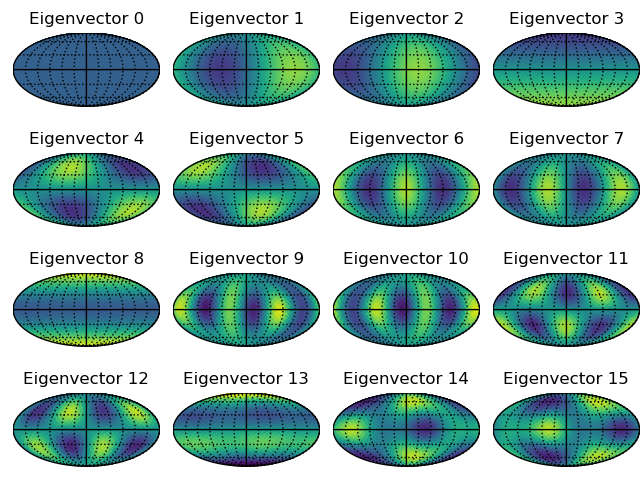
\includegraphics[width=0.6\textwidth]{../codes/03.FEM_laplacian/HEALPix/img/linear_FEM_8_eigenvectors.png}	
		\label{fig:spherical harmonics}
		\caption{The first 16 spherical harmonics}
	\end{figure}
	
	\item Of all the possible basis for $L^2(S^2)$ the spherical harmonics uniquely exploit the symmetries of the sphere. Under a rotation $g$, each spherical harmonic of degree $l$ is transformed into a linear combination of only those spherical harmonics of same degree $l$.
	Thus the effect of a rotation on a function expressed in the basis of the spherical harmonics is a multiplication by a semi-infinite block-diagonal matrix with the $(2l+1)\times(2l+1)$ blocks for each $l \geq 0$ given by $$D^{(l)}(g) = \left(D^{(l)}_{m,n}\right) (g) =  \left(D^{(l)}_{m,n}\right)(u(\phi)a(\theta)u(\psi)) = e^{-im\psi}d^{(l)}_{m,n}(\cos \theta) e^{-in\phi}$$
	The effect of all of this is to block-diagonalize rotationally invariant operators; namely, convolution operators obtained as weighted averages of the rotation operators by functions or kernels. For example the Laplace-Beltrami operator, that acts diagonally on the spherical harmonic basis.
	\item \begin{definition}{[\textit{Left Convolution}]}\\
		$k\star f(\omega) = \left(\int_{g\in SO(3)}dg\ k(g\eta)\Lambda(g)\right)f(\omega) = \int_{g\in SO(3)}k(g\eta)f(g^{-1}\omega)dg$
		where $\eta$ is the north pole. 
	\end{definition}
	Since the convolution is a linear combination of rotation operators $\Lambda(g)$, it follows that also the convolution must be block diagonalized. Indeed,
	$$\hat {(f \star h)}(l,m) = 2\pi \sqrt{\frac{4\pi}{2l+1}}\hat f(l,m) \hat h(l,0) $$

\end{enumerate}

\subsection{Spherical Convolutional Neural Networks}
[Review of \textit{Spherical CNNs}]
\subsection{Graph Spectral Theory} \label{sec:Chapter1: Spectral Graph Theory}
[Review of \textit{The emerging field of Graph Signal Processing}]
\subsection{Deep Sphere V1.0}
[Review of \textit{Deep Sphere}]
\subsection{Belkin's trinity}
[Review of \textit{the Belkin's trinity}]

\subsubsection{Towards a theoretical foundation of Laplacian-based manifold methods}
In this paper they present two results: a pointwise probabilistic convergence of \textbf{the extension of the graph Laplacian} 
\begin{definition}{Graph Laplacian}
	$$ \left(\mathbf L_n^t\right)_{ij}=\begin{cases}
	-w_{ij}, & i\neq j\\
	\sum_{k}w_{ik}, & i=j
	\end{cases}$$
\end{definition}
\begin{definition}{Point cloud Laplace operator}
	$$L_n^t:\quad(L_n^tf)(y) = \frac{1}{n}f(y)\sum_i e^{-\frac{||x_i-y||^2}{4t}}-\frac{1}{n}\sum_ie^{-\frac{||x_i-y||^2}{4t}}f(x_i)$$
\end{definition}
\begin{definition}{Functional approximation to the Laplace-Beltrami operator} \label{eq:L^t}
	$$L^tf(p) :=  \frac{1}{ (4\pi t)^{\frac{k+2}{2}}} \int_\mathcal Me^{-\frac{||p-x||^2}{4t}}\left(f(x)-f(p)\right)d\mu(x)$$
\end{definition}

\begin{theorem}{Pointwise convergence}
	$$\forall f \in C^\infty(\mathcal M)\quad  C\frac{(4\pi t_n)^{-\frac{k+2}{2}}}{n} L_n^t f(\bf x) \xrightarrow{n\to\infty}\triangle_\mathcal M f(\bf x)$$
\end{theorem}


and a uniform (pointwise convergence of the operator) one
\begin{theorem}{uniform convergence}
	$$\sup_{x\in\mathcal M, f\in \mathcal F_C}\left| C\frac{(4\pi t_n)^{-\frac{k+2}{2}}}{n} L_n^t f(\bf x) - \triangle_\mathcal M f(\bf x) \right|\xrightarrow{n\to\infty}0
	, \quad \mathcal F_C = \left\{f\in C^\infty(\mathcal M), f^{(i)}(x)\leq M, i=1,2,3\right\}$$
\end{theorem}


here nothing is said about convergence of the spectra, plus there's nothing written about the relationship between $\mathbf{Eig} L_n^t$ (the eigenfunctions and eigenvalues of the extension of the graph Laplacian) and $\mathbf {Eig} \mathbf {L}_n^t$ (the eigenvectors and eigenvalues of the matrix Laplacian).

Theorem 1 is proven by simple analysis arguments and by Hoeffding's formula (probability). 
First, by the simple law of large numbers, we have that for a fixed $t>0$, a fixed function $f$ and a fixed point $p\in\mathcal M$
\begin{equation}\label{eq:pointwise convergence of laplacian discrete approximation}
	\lim_{n\to\infty}\frac{1}{tn}\frac{1}{ (4\pi t)^{\frac{k}{2}}}L_n^tf(p)= L^tf(p)
\end{equation}




To prove the convergence of $L^t$ to $\triangle_\mathcal M$, then we need three steps, that we can recycle completely. They use the fact that thanks to the exponential map the heat kernel centered on $p$ on any manifold can be approximated by a Gaussian in the ambient Euclidean space in a small neighborhood of $p$, and the relationship between Euclidean distances and geodesic distances.

Theorem 2 is proven with arguments of Functional Analysis: Ascoli-Arzelà, compact convergence in Sobolev spaces, etc.etc...

\subsubsection{Consistency of Spectral Clustering}
$$ \mathbf{Eig} \mathbf{L}^t_n \xrightarrow[a.s.]{n\to\infty} \mathbf{Eig} L^t $$
It aims at proving the convergence of eigenvalues and eigenvectors of random graph Laplacian matrices for growing sample size. They present two results: one for the normalized Laplacian and one for the unnormalized Laplacian. Since the matrix eigenvectors grow in dimension as the sample size increases, standard convergence arguments can not be applied. However, they show that there exists a function $f\in C(\mathcal M)$ such that the difference between the eigenvector $v_n$ and the restriction of $f$ to the sample converges to $0$

$$||v_n-\rho_nf||\rightarrow 0$$

To do so they see the eigenvector $v_n$ as the restriction to the sample of a continuous eigenfunction $f_n$ of some continuous operator $U'_n$ that acts on the space $C(\mathcal M)$. Then they use the fact that 

$$||v_n-\rho_nf||_\infty = ||\rho_nf_n-\rho_nf||_\infty\leq ||f_n-f||_\infty$$


So, it will just be necessary to show that  $$||f_n-f||_\infty\rightarrow 0$$
\textbf{compact convergence} of both matrices towards $L^t$ (where $\mathcal M$ is a compact metric space) in the Banach space of the continuous functions $(C, ||\cdot||_\infty)$. 

Compact convergence ensures convergence of spectral properties in the following sense: for isolated eigenvalues of the limit operator $\triangle_\mathcal M$ with finite multiplicity we have convergence of eigenvalues and eigenspaces but not convergence of eigenfunctions. for isolated simple eigenvalues of the limit operator we have also convergence of the eigenfunctions!

The proof consists in three steps:
\paragraph{Step 1} Construct a bounded operator $U'_n$ on the Banach space $(C(\mathcal M), ||\cdot||_\infty)$ such that restricted on the sampled values behaves like $\mathbf{L}'_n$. Then, construct an operator $U'$ such that for the law of large numbers for a fixed $f$ and for a fixed $x$, $U'_nf(x) \xrightarrow U'f(x) $
\paragraph{Step 2} Here they establishes the connection between the spectra of $L'_n$ and $U'_n$. In particular, they prove a one-to-one correspondence between the eigenfunctions and eigenvalues of $U'_n$ and the eigenvectors and eigenvalues of $L'_n$, provided that satisfy $\lambda\notin \{1\}=\sigma_{ess}(U'_n)= \sigma_{ess}(U')$.
\paragraph{Step 3} Here we prove compact convergence:

$$U'_n \xrightarrow[n\to\infty]{c,\ a.s.}U'$$

At the light of compact convergence and on the analysis of the essential spectrum of $U'_n, U'$ and the one-to-one correspondence of the spectra done in step 2, given Proposition 6 \textit{Perturbation results for compact convergence} we get to the following result

\begin{theorem}
	Let $\lambda\neq 1 $ be an eigenvalue of $U'$ and $M\subset \mathbb C$ an open neighborhood of $\lambda$ such that $\sigma(U')\cap M=\{\lambda\}$. Then:
	\begin{enumerate}
		\item Convergence of eigenvalues: The eigenvalues in$\sigma(L'_n)\cap M$ converge to $\lambda$ in the sense that every sequence $(\lambda_n)_{n\in\mathbb N}$ with $\lambda_n\in\sigma(L'_n)\cap M$ satisfies $\lambda_n\rightarrow \lambda$ almost surely.
		\item Convergence of spectral projections: There exists some $N\in\mathbb N$ such that for $n>N$, the sets $\sigma(U'_n)\cap M$ are isolated in $\sigma(U'_n)$. For $n>N$, let $Pr'_n$ be the spectral projection of $U'_n$ corresponding to $\sigma(U'_n)\cap M$, and $Pr$ the spectral projection of $U$ for $\lambda$. Then $Pr'_n\xrightarrow p Pr a.s.$
		\item Convergence of eigenvectors: if $\lambda$ is a single eigenvalue, then the eigenvectors of $L'_n$ converge a.s. up to a change of sign: if $v_n$ is the eigenvector
		of $L'_n$ with eigenvalue $\lambda_n$, $v_{n,i}$ its i-th coordinate, and $f$ the eigenfunction of eigenvalue $\lambda$, then there exists a sequence $(a_n)_{n\in\mathbb N}$ with $a_i \in \{+1,-1\}$ such that $\sup_{i=1,...,n} |a_nv_{n,i} - f(X_i)| \rightarrow 0$ a.s. In particular, for all $b \in\mathbb R$, the sets $\{a_nf_n > b\}$ and $\{f > b\}$ converge, that is, their symmetric difference satisfies $P(\{f > b\}\triangle\{a_nf_n > b\}) \rightarrow 0$.
	\end{enumerate}
\end{theorem}

A similar theorem is stated also for non-normalized Laplacian matrix, although the arguments stay the same.
\subsubsection{Convergence of Laplacian Eigenmaps}
Here all the pieces are put together. 

$$ \mathbf{Eig} \mathbf{ L}^t_n \xrightarrow[a.s.]{n\to\infty} \mathbf{Eig} L^t \xrightarrow{t\to0} \mathbf{Eig} \triangle_\mathcal M $$

\begin{theorem}
	Let $\lambda_{n,i}^t$ be the ith eigenvalue of $\hat L_n^t$ and $e^t_{n,i}$ be the corresponding eigenfunction (which for each fixed i will be shown to exist for t sufficiently small). Let $\lambda_{i}$ be the ith eigenvalue of $\triangle_\mathcal M$ and $e_{i}$ be the corresponding eigenfunction. Then there exists a sequence $t_n\rightarrow 0$ such that
	
	$$\lim_{n\rightarrow\infty} \lambda_{n,i}^{t_n}=\lambda_i$$
	$$\lim_{n\rightarrow\infty}||e_{n,i}^{t_n}(x) - e_i(x)||_2 = 0$$
	
	where the limits are in probability.
	
\end{theorem}

\paragraph{Step 1: Spectral convergence of the empirical approximation $\mathbf{ L}_n^t$ to $L^t$}
Recycle the work of \textbf{Consistency of Spectral Clustering} with the analysis of the essential spectrum of the limit operator $\sigma_{ess}(L^t)$.
\paragraph{Step 2: Spectral convergence of the functional approximation $L^t$ to $\triangle$}
Really hard. Uniform operator convergence does not hold, however spectral convergence is still assured in theorem 4.1 of the paper. This part, although really hard, will stay the same!
sub

\pagebreak


%*******************************************************************************
%*********************************** First Chapter *****************************
%*******************************************************************************
%!TEX root = 0.main.tex

\section{Improving Deep Sphere}
\subsection{Adapting Belkin's setting to HEALPix sampling}
\subsubsection*{Pointwise convergence of the Graph Laplacian in the HEALPix case}
\subsubsection*{About the kernel width $t$}
Here we discuss how a big $t$ better captures the low frequencies, a smaller one captures the high frequencies up to the nearest neighbors.
\subsubsection*{Reducing the number of neighbors}
Here we present our final result obtained by thresholding the weights
\subsection{Experimental validation}
Here we report Frederick's results with the two different constructions


\pagebreak


%*******************************************************************************
%*********************************** Second Chapter ***************************
%*******************************************************************************
%!TEX root = 0.main.tex

\section{Other samplings and other Discrete Laplacians}

[What we want from the Laplacian matrix]\\
In a Graph Spherical CNN we use the fact that when the sampling of the sphere is regular enough, the graph $W_{i j} = \exp {-\frac{\norm{x_i-x_j}^2}{4t}}$ is such that the corresponding graph Laplacian $\mathbf L_n^t=D-W$ has a spectrum that is close enough to the spectrum of $\triangle$ so that we can approximate a spherical convolution of a signal with a kernel with a multiplication of a polynomial of the discrete Laplacian $\sum_k \theta_k (\mathbf L_n^t)^k$ times the vector of the sampled signal $\mathbf f_i = f(x_i)$. 

[Stating the problem we want to solve]\\
In Chapter 2 we showed a way to construct $\mathbf L_n^t$ that well approximates $\triangle$ in the case of a much regular sampling of the sphere, HEALPix. In this Chapter we focus to others samplings less uniform than HEALPix. The sampling that we will use for our study, very used in applications, is the so called equiangular sampling. We will observe that in this case the Heat Kernel Graph Laplacian matrix is not able to correctly approximate the continuous Laplace-Beltrami operator, due to the fact that the equiangular sampling samples some specific areas of the sphere more than others. The goal of this chapter is to find a way of building a discrete approximation $\mathbf L$ of the Laplace-Beltrami operator more robust to non uniform sampling than the Heat Kernel Graph Laplacian matrix $\mathbf L_n^t$ used so far.

[Say what we did to solve it]\\
This chapter is organized as follows: In Section \ref{sec:Chapter3: Heat Kernel Graph Laplacian on the Equiangular Sampling} we introduce the equiangular sampling and the results that we obtained with the Heat Kernel Graph Laplacian matrix. In Section \ref{sec:Chapter3: other discrete laplacians} we present a short overview of different ways of building an discrete approximation of the Laplace-Beltrami operator; in Section \ref{sec:Chapter3: Using the Finite Element Method to approximate the Laplace-Beltrami operator on a manifold} we deepen how to use the Finite Element Method (FEM) to construct a discrete approximation of $\triangle$ and how this way of constructing $\mathbf L$  is actually capable of taking into account the non uniformity of the sampling and correct it. in Section \ref{sec:Chapter3: Results} we present and discuss the results obtained.
\subsection{Heat Kernel Graph Laplacian on the Equiangular Sampling}
\label{sec:Chapter3: Heat Kernel Graph Laplacian on the Equiangular Sampling}

\subsubsection{The Equiangular Sampling}
[Present the equiangular sampling]\\
Given the usual parametrization $x = x(\theta, \phi)$ of the sphere
$$
\mathbb{S}^{2}=\left\{x=\left(x_{1}, x_{2}, x_{3}\right) \in \mathbb{R}^{3} :\|x\|_{\mathbb{R}^{3}}=\left(x_{1}^{2}+x_{2}^{2}+x_{3}^{2}\right)^{1 / 2}=1\right\}
$$

$$
x_{1}=\cos (\phi) \sin (\theta), \quad x_{2}=\sin (\phi) \sin (\theta), \quad x_{3}=\cos (\theta)
$$
Let $m\in\mathbb N$, the uniform sampling of bandwidth $b=2^m$ is given by 
$
x_{j k}^{(b)}=x\left(\theta_{j}^{(b)}, \phi_{k}^{(b)}\right)
$
where
$$
\theta_{j}^{(b)} :=\pi \frac{j}{2 b}, \quad \phi_{k}^{(b)} :=2 \pi \frac{k}{2 b}
$$
\begin{figure}[h!]
	\centering
	\label{fig:equiangular sampling}
	\caption{Equiangular sampling with bandwidth $n=16$}
	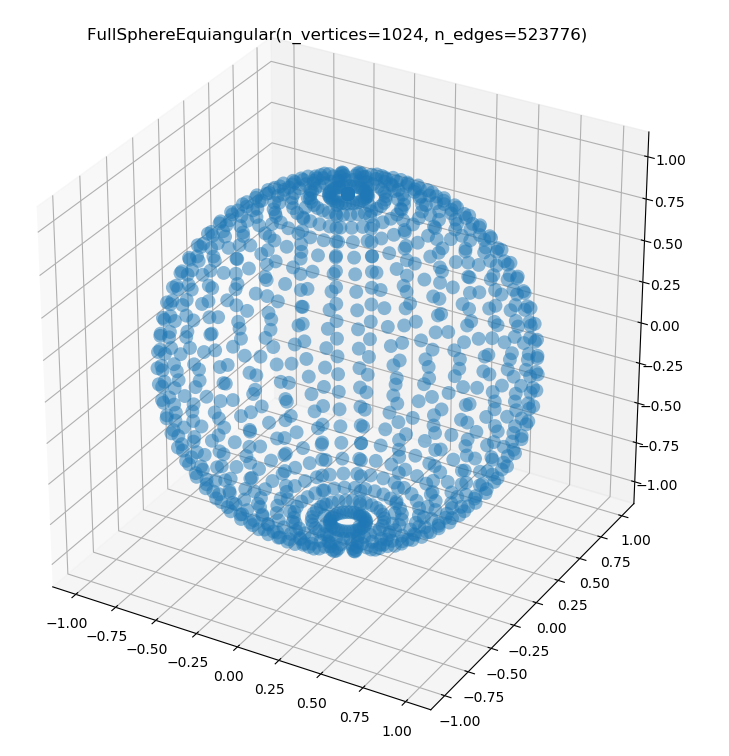
\includegraphics[width=0.5\textwidth]{../codes/02.HeatKernelGraphLaplacian/equiangular/equiangular.png}
\end{figure}
One has $n=4b^2$ points on the sphere, where $x_{0 k}^{(b)}$ corresponds to the north pole for every $k$. Notice also that the south pole is never sampled. In figure \ref{fig:equiangular sampling} it can also be appreciated how the area close to the poles is much more sampled that the equator. One reason for which this sampling is very useful is the following result from \cite{Driscoll:1994:CFT:184069.184073}, that states that any band limited function can be exactly recovered from its sampled values $f\left(x_{j k}^{(b)}\right)$:
\vspace{0.5cm}
\begin{prop}\label{prop:equiangular sampling theorem}
	Let \(l_{0} \in \mathbb{N}\) and \(m_{0} \in \mathbb{Z},\left|m_{0}\right| \leq l_{0} .\) If \(f=\sum_{l=0}^{b-1} \sum_{m=-l}^{l} \widehat{f}(l, m) Y_{l}^{m}\)
	then
	
	$$
	\begin{aligned} \widehat{f}\left(l_{0}, m_{0}\right)=& \frac{1}{4 b^{2}} \sum_{j=0}^{2 b-1} \sum_{k=0}^{2 b-1} f\left(x_{j k}^{(b)}\right) \overline{Y_{l_{0}}^{m_{0}}\left(x_{j k}^{(b)}\right)} \sin \left(\theta_{j}^{(b)}\right) \times \\ & \times \frac{4}{\pi} \sum_{l=0}^{b-1} \frac{1}{2 l+1} \sin \left((2 l+1) \theta_{j}^{(b)}\right) \end{aligned}
	$$
\end{prop}
\vspace{0.5cm}

\subsubsection{Heat Kernel Graph Laplacian}
Thanks to Proposition \ref{prop:equiangular sampling theorem}, assuming we can compute the Fourier transform of the eigenvectors of the Heat Kernel Graph Laplacian matrix and see how much they are aligned with the eigenspaces of the true Laplace-Beltrami operator. Here the results:


\begin{table}[h!]
	\centering
	\label{table:equiangular kernel width}
	\caption{Kernel width $t$ used to construct the Heat Kernel Graph Laplacian matrix fr each bandwidth $b$}
	\begin{tabular}{ c|c } 
	
$b$ & $t$ \\ 
	\hline
4 & 0.5 \\ 
8 & 0.3 \\ 
16 & 0.1 \\ 
	
	\end{tabular}
\end{table}

\begin{figure}[h!]
	\centering
	\label{fig:equiangular sampling alignment}
	\caption{Alignment of eigenspaces of the Heat Kernel Graph Laplacian matrix with the true Laplace-Beltrami eigenspaces on the equiangular sampling with $b=16$ and kernel width $t=0.1$}
	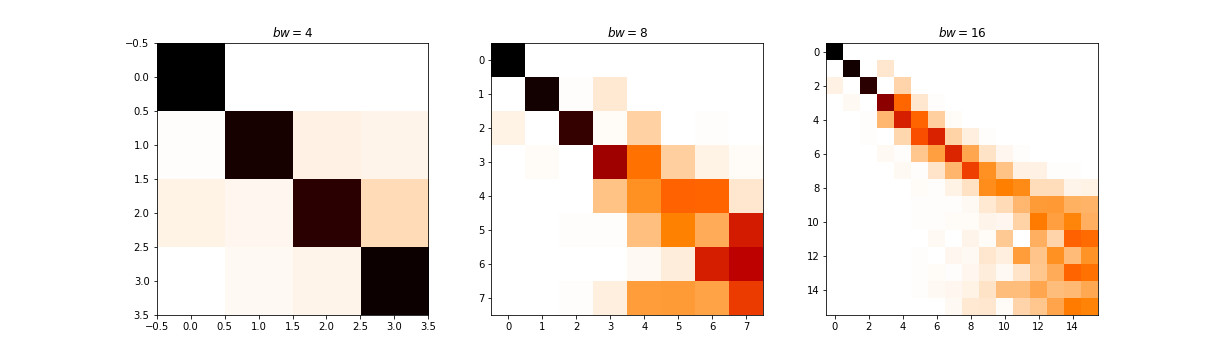
\includegraphics[width=0.9\textwidth]{../codes/02.HeatKernelGraphLaplacian/equiangular/equi_full.png}
\end{figure}
\begin{figure}[h!]
	\centering
	\label{fig:equiangular sampling alignment diagonal}
	\caption{Alignment of eigenspaces of the Heat Kernel Graph Laplacian matrix with the true Laplace-Beltrami eigenspaces on the equiangular sampling}
	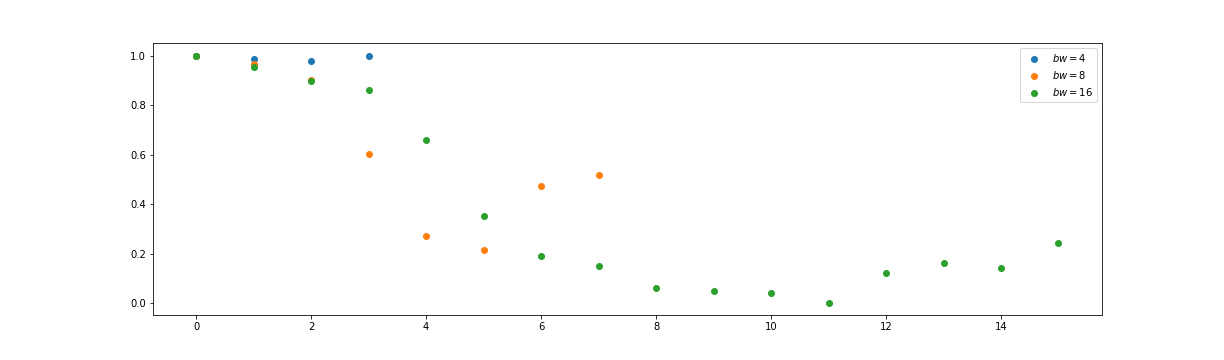
\includegraphics[width=0.9\textwidth]{../codes/02.HeatKernelGraphLaplacian/equiangular/equi_full_diagonal.png}
\end{figure}
\begin{figure}[h!]
	\centering
	\label{fig:equiangular sampling alignment eigenvalues}
	\caption{Eigenvalues of the Heat Kernel Graph Laplacian matrix on the equiangular sampling with $b=16$ and kernel width $t=0.1$}
	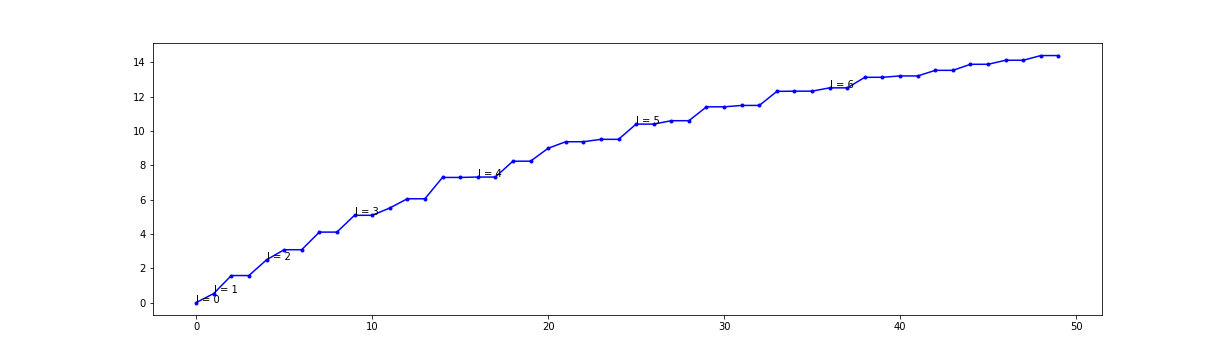
\includegraphics[width=0.9\textwidth]{../codes/02.HeatKernelGraphLaplacian/equiangular/equi_full_eigenvalues_16.png}
\end{figure}

It can be appreciated how poor these results are compared to the ones obtained with the HEALPix sampling. \\

[ Explain why they are so bad: Perspective of the quadrature formula]\\
A way to understand what's going on is the following: remembering the proof of theorem \ref{theo:pointwise convergence in the healpix case} and using again the notation $\phi^{t}(x ; y)=e^{-\frac{||x-y||^2}{4t}}\left(f(y)-f(x)\right)$, the key thing is to make $L_n^tf(y)=\sum_i \frac{1}{n} \phi^{t}(x_i ; y)$  approximate $L^tf(y)=\int_\mathcal M\phi^{t}(x ; y)d\mu(x)$, in other words we can see the graph weights as \textit{quadrature weights} meant to approximate the continuous integral on the right hand side of equation \ref{eq:quadrature approximation}.
\begin{equation}
\label{eq:quadrature approximation}
	\sum_i \frac{1}{n} \phi^{t}(x_i ; y) \quad \approxeq\quad \int_\mathcal M\phi^{t}(x ; y)d\mu(x)
\end{equation}
The way of building the graph of Belkin et al. works in the case of random sampling because in that way the sampling in the limit of the SLLN will sample the manifold uniformly, and thus there's no need of re-weighting the graph; in case of non uniform sampling, we intuitively need to modify the Heat Kernel weights $W_{i j}=e^{-\frac{\norm{x_i-x_j}^2}{4t}}$ with some coefficients $\alpha_i$ to create a re-weighted graph 
$$
W'_{i j} = \alpha_i W_{i j}
$$

in order for $L_n^tf(y)$ to correctly approximate $L^tf(y)$, where $\alpha_i$ would be smaller in pixels that are in areas closer to the poles and bigger in areas closer to the equator. 

\begin{equation}
\label{eq:quadrature approximation 2}
\sum_i \frac{1}{n} \alpha_i \phi^{t}(x_i ; y) \quad \approxeq\quad \int_\mathcal M  \phi^{t}(x ; y)d\mu(x)
\end{equation}
In the next section we present some different ways of building the matrix $\mathbf L$.

\clearpage
\subsection{Other Discrete Laplacians}\label{sec:Chapter3: other discrete laplacians}
Present all the other ways of approximating the Laplace-Beltrami operator you found: graphs, Laplace de Rham, FEM
\subsubsection{Frossard/Khasanova graph}
\begin{figure}[h]
	\label{fig:Frossard/Khasanova graph}
	\centering
	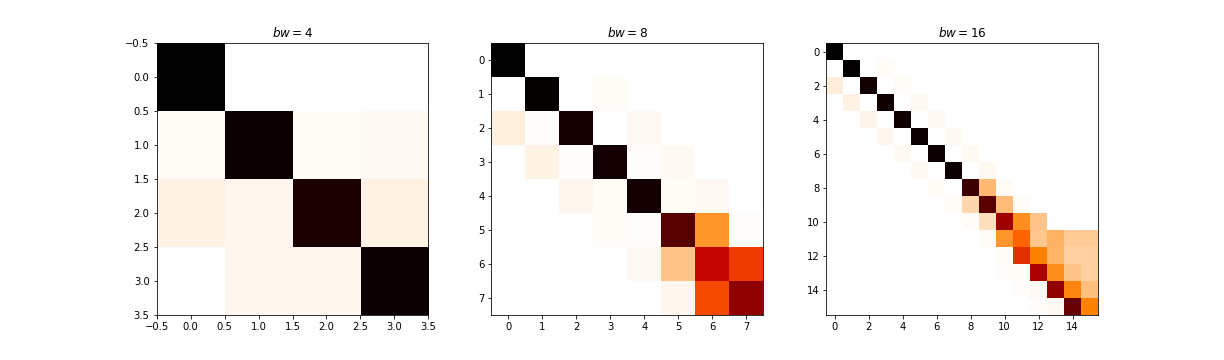
\includegraphics[width=0.9\textwidth]{../codes/02.HeatKernelGraphLaplacian/equiangular/equi_Khasanova_Frossard_full.png}
	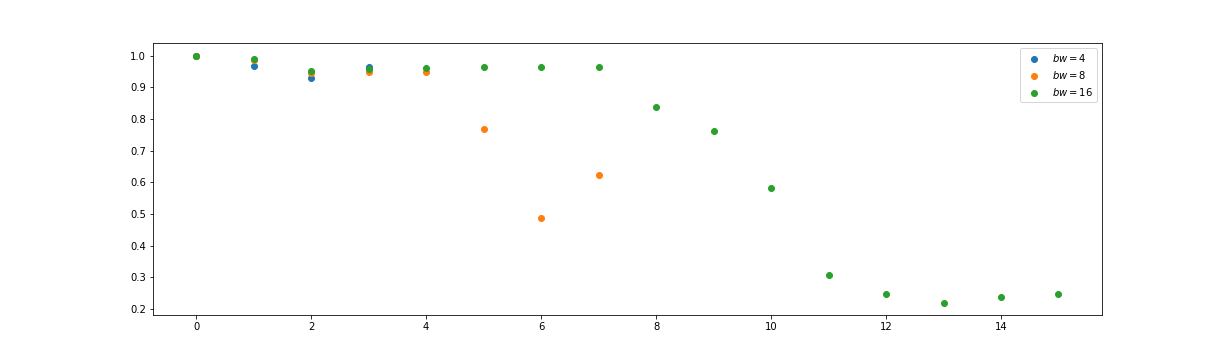
\includegraphics[width=0.9\textwidth]{../codes/02.HeatKernelGraphLaplacian/equiangular/equi_Khasanova_Frossard_full_diagonal.png}
	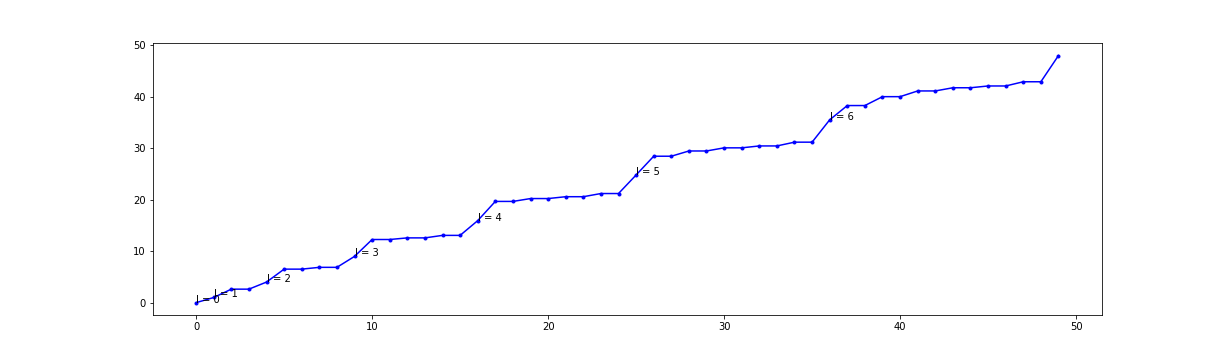
\includegraphics[width=0.9\textwidth]{../codes/02.HeatKernelGraphLaplacian/equiangular/equi_full_Khasanova_Frossard_eigenvalues_16.png}
	\caption{Frossard/Khasanova graph}
\end{figure}
\begin{figure}[h]
	\label{fig:Frossard/Khasanova geodesic graph}
	\centering
	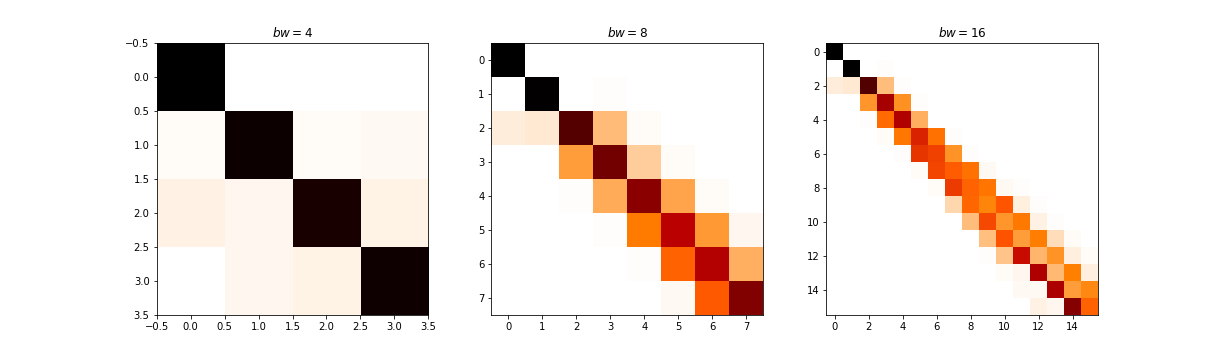
\includegraphics[width=0.9\textwidth]{../codes/02.HeatKernelGraphLaplacian/equiangular/equi_Khasanova_Frossard_full_geodesic.png}
	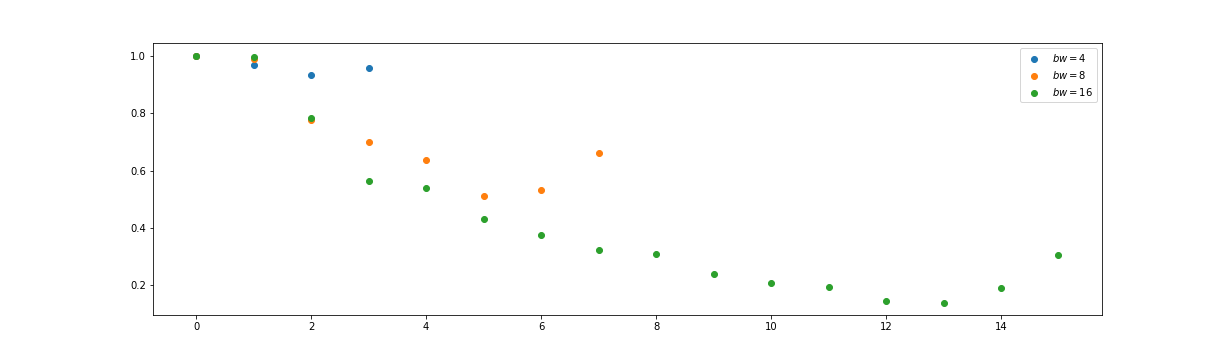
\includegraphics[width=0.9\textwidth]{../codes/02.HeatKernelGraphLaplacian/equiangular/equi_Khasanova_Frossard_full_diagonal_geodesic.png}
	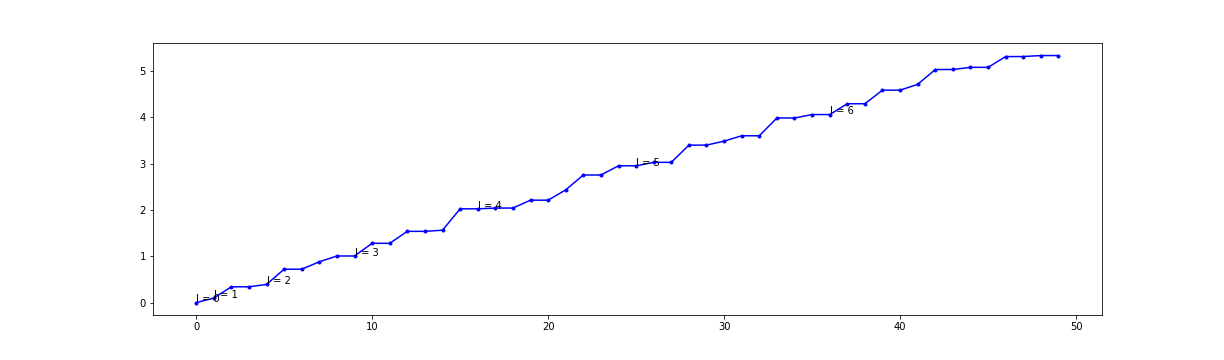
\includegraphics[width=0.9\textwidth]{../codes/02.HeatKernelGraphLaplacian/equiangular/equi_full_Khasanova_Frossard_eigenvalues_16_geodesic.png}
	\caption{Frossard/Khasanova geodesic graph}
\end{figure}
\subsection{Using the Finite Element Method to approximate the Laplace-Beltrami operator on a manifold}\label{sec:Chapter3: Using the Finite Element Method to approximate the Laplace-Beltrami operator on a manifold}
Basic ingredients: works on a mesh, 
\subsubsection{Galerkin Method and Finite Element Method}
General introduction to the FEM: definitions, weak formulation, functional spaces, Galerkin method, linear FEM.
\subsubsection{The eigenvalue problem on a manifold}
Weak formulation of the eigenvalue problem on the sphere, generalized eigenvalue problem, lumping of the mass matrix, discussion on the solvers
\begin{figure}[h]
	\label{fig:Lumping}
	\centering
	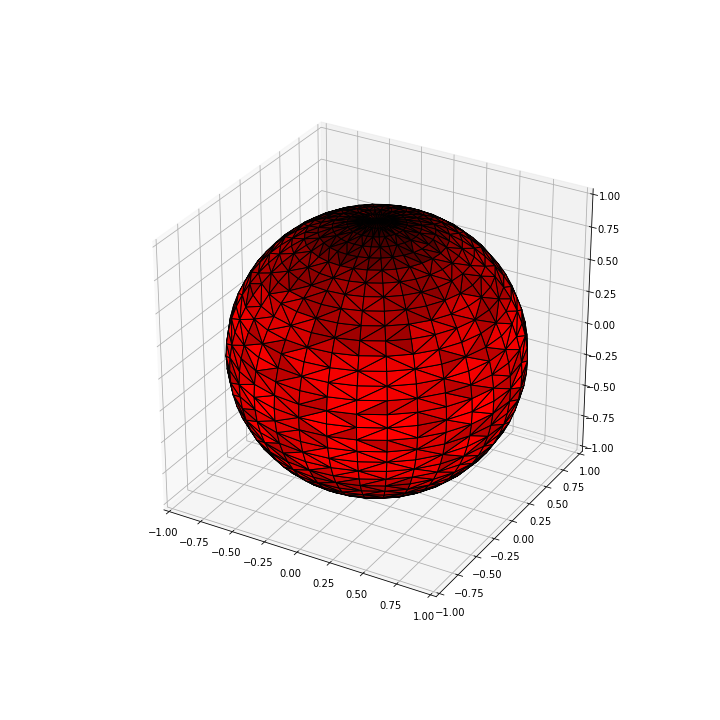
\includegraphics[width=0.9\textwidth]{../codes/03.FEM_laplacian/equiangular/normal/img/mass_matrix_diagonal.png}

	\caption{Diagonal of the lumped mass matrix}
\end{figure}
\subsection{Results}
\label{sec:Chapter3: Results}

\subsubsection{Alignment of eigenspaces and analysis of the spectra}

\paragraph{HEALPix}
\begin{figure}[h]
	\label{fig:HeatKernelGraphLaplacianHealpix}
	\centering
	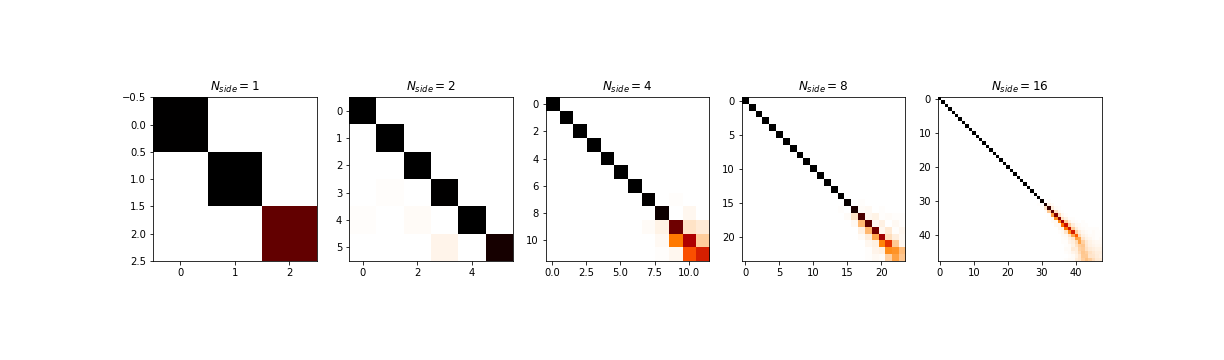
\includegraphics[width=0.9\textwidth]{../codes/02.HeatKernelGraphLaplacian/HEALPix/06_figures/optimal_thresholded.png}
	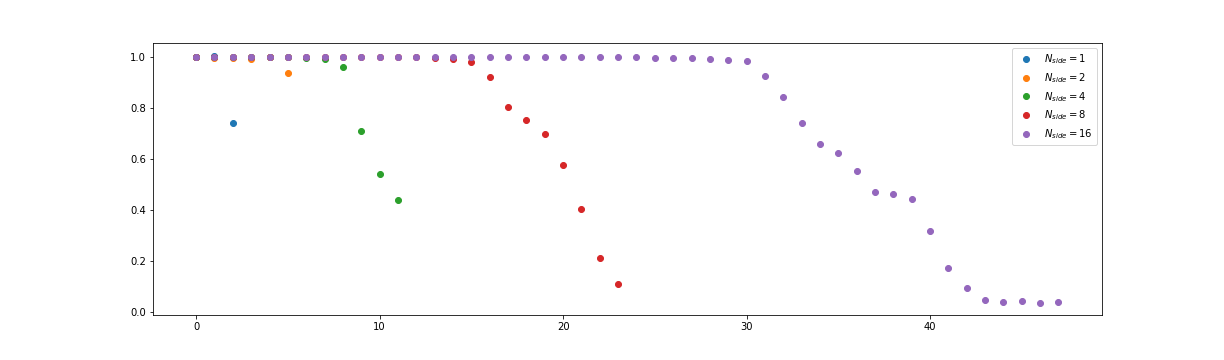
\includegraphics[width=0.9\textwidth]{../codes/02.HeatKernelGraphLaplacian/HEALPix/06_figures/optimal_thresholded_diagonal.png}	
	\caption{Heat Kernel Graph Laplacian on HEALPix}
\end{figure}

\begin{figure}[h]
	\label{fig:FEMHealpix}
	\caption{Linear FEM Laplacian on HEALPix}
	\centering
	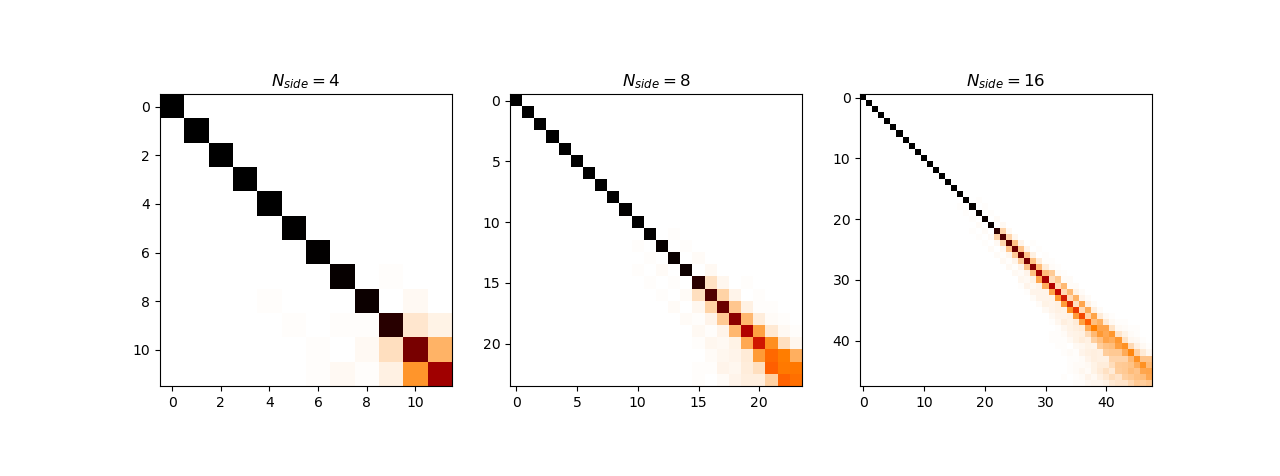
\includegraphics[width=0.8\textwidth]{../codes/03.FEM_laplacian/HEALPix/img/linearFEM.png}
	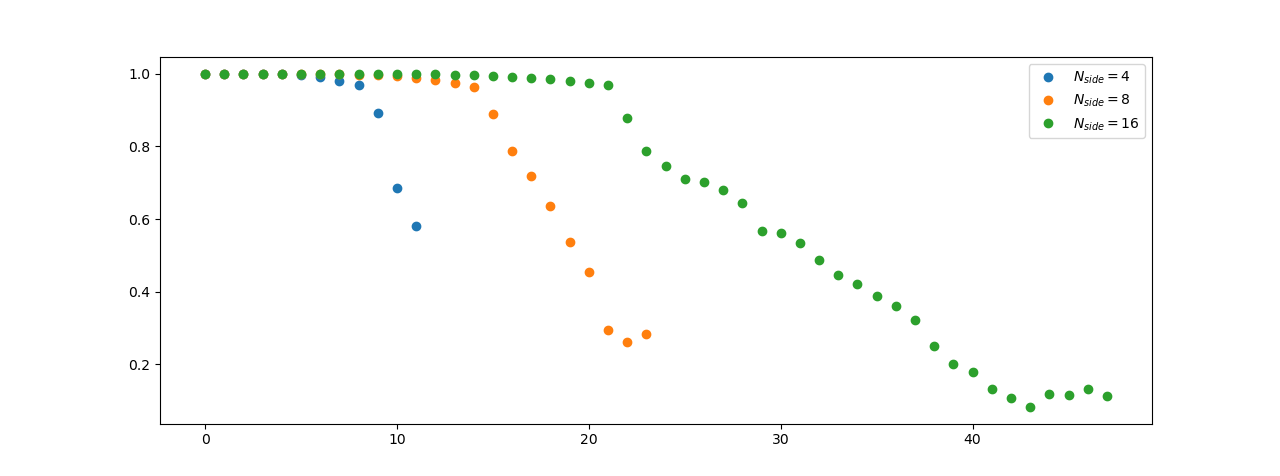
\includegraphics[width=0.8\textwidth]{../codes/03.FEM_laplacian/HEALPix/img/linearFEM_diagonal.png}	
	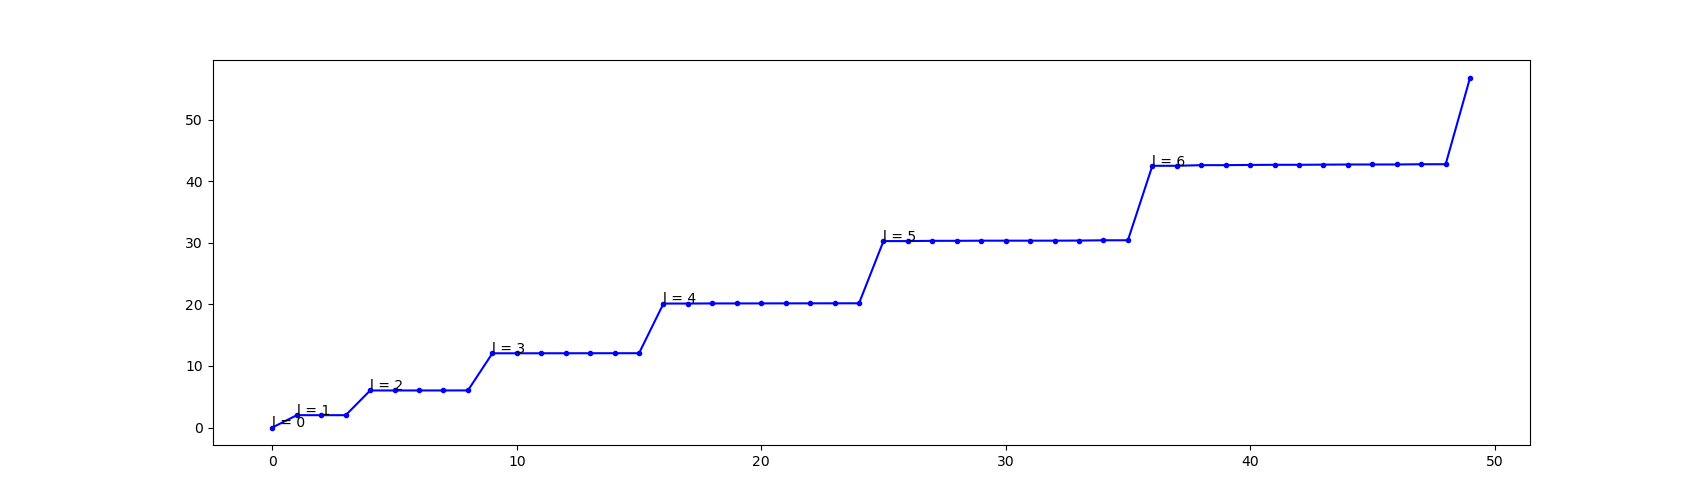
\includegraphics[width=0.8\textwidth]{../codes/03.FEM_laplacian/HEALPix/img/FEM_eigenvalues_16.png}	 
\end{figure}

\paragraph{Equiangular}
\begin{figure}[h]
	\label{fig:HeatKernelGraphLaplacianEquiangular}
	\caption{Heat Kernel Graph Laplacian on equiangular sampling}
	\centering
	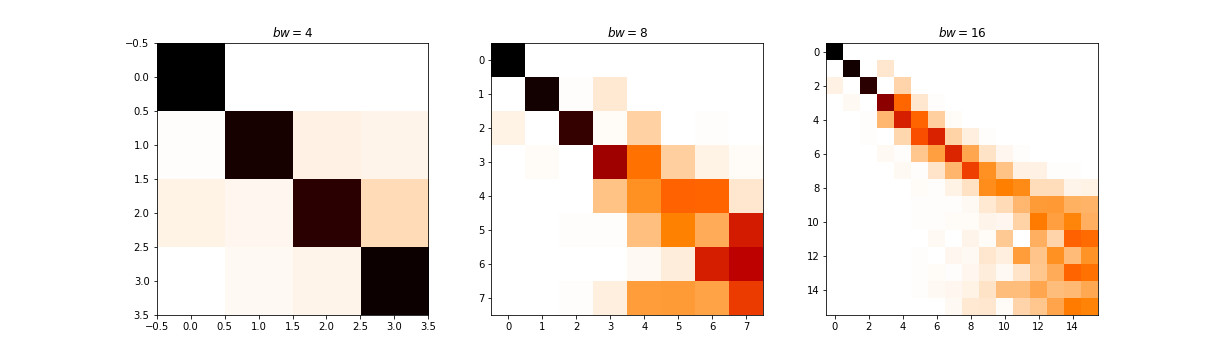
\includegraphics[width=0.9\textwidth]{../codes/02.HeatKernelGraphLaplacian/equiangular/equi_full.png}
	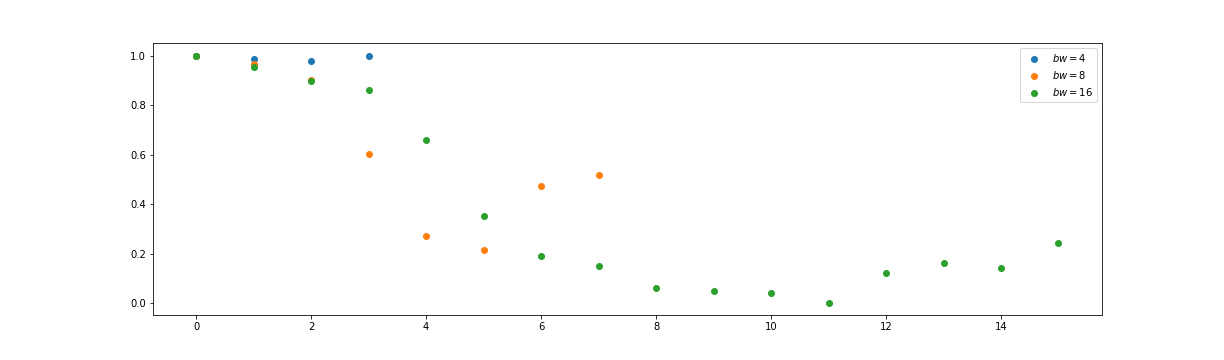
\includegraphics[width=0.9\textwidth]{../codes/02.HeatKernelGraphLaplacian/equiangular/equi_full_diagonal.png}	
	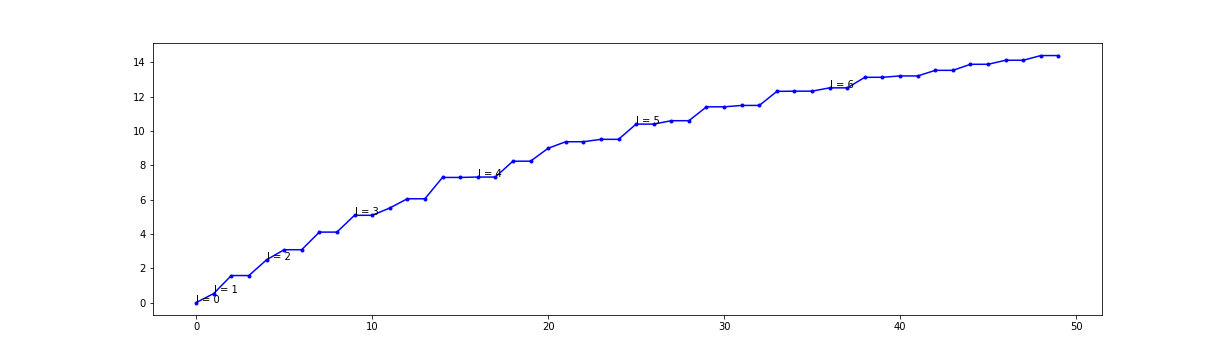
\includegraphics[width=0.9\textwidth]{../codes/02.HeatKernelGraphLaplacian/equiangular/equi_full_eigenvalues_16.png}	
\end{figure}


\begin{figure}[h]
	\label{fig:FEMequiangular}
	\caption{Linear FEM Laplacian on equiangular sampling}
	\centering
	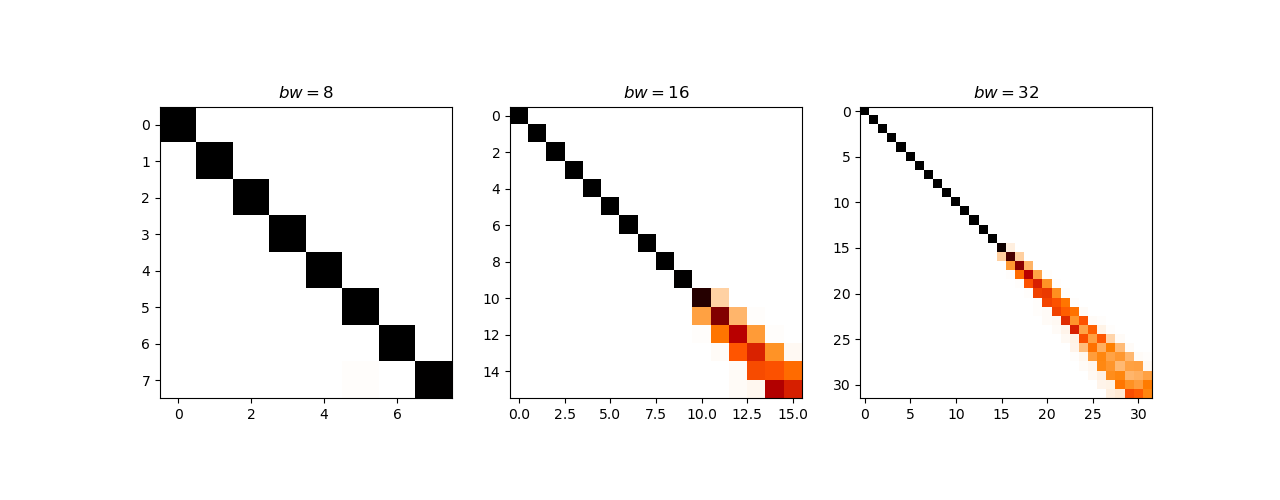
\includegraphics[width=0.9\textwidth]{../codes/03.FEM_laplacian/equiangular/normal/img/linearFEM.png}
	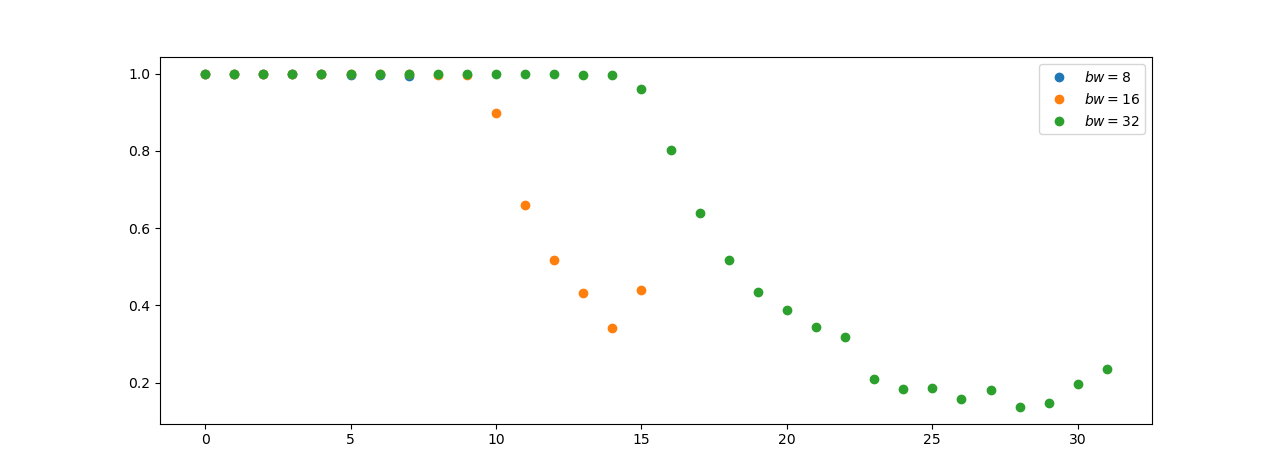
\includegraphics[width=0.9\textwidth]{../codes/03.FEM_laplacian/equiangular/normal/img/linearFEM_diagonal.png}	
	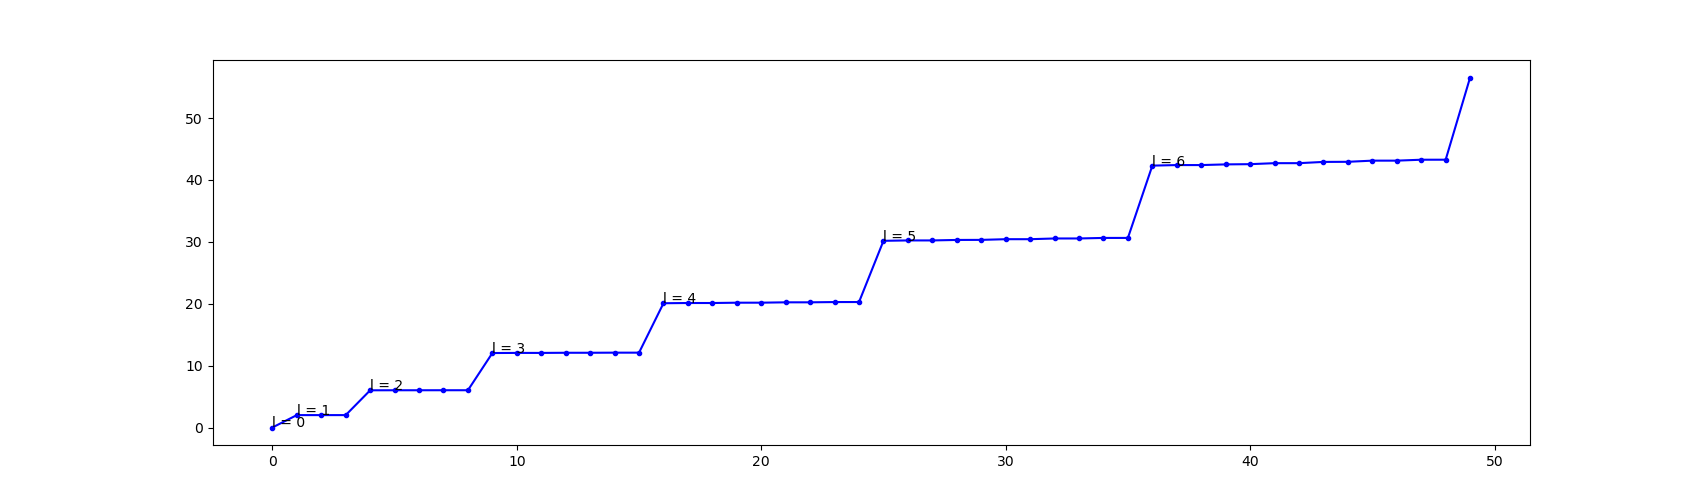
\includegraphics[width=0.9\textwidth]{../codes/03.FEM_laplacian/equiangular/normal/img/FEM_eigenvalues_16.png}	
\end{figure}

\paragraph{Lumping the mass matrix}


\begin{figure}[h]
	\label{fig:FEMequiangularLumped}
	\caption{Lumped Linear FEM Laplacian on equiangular sampling}
	\centering
	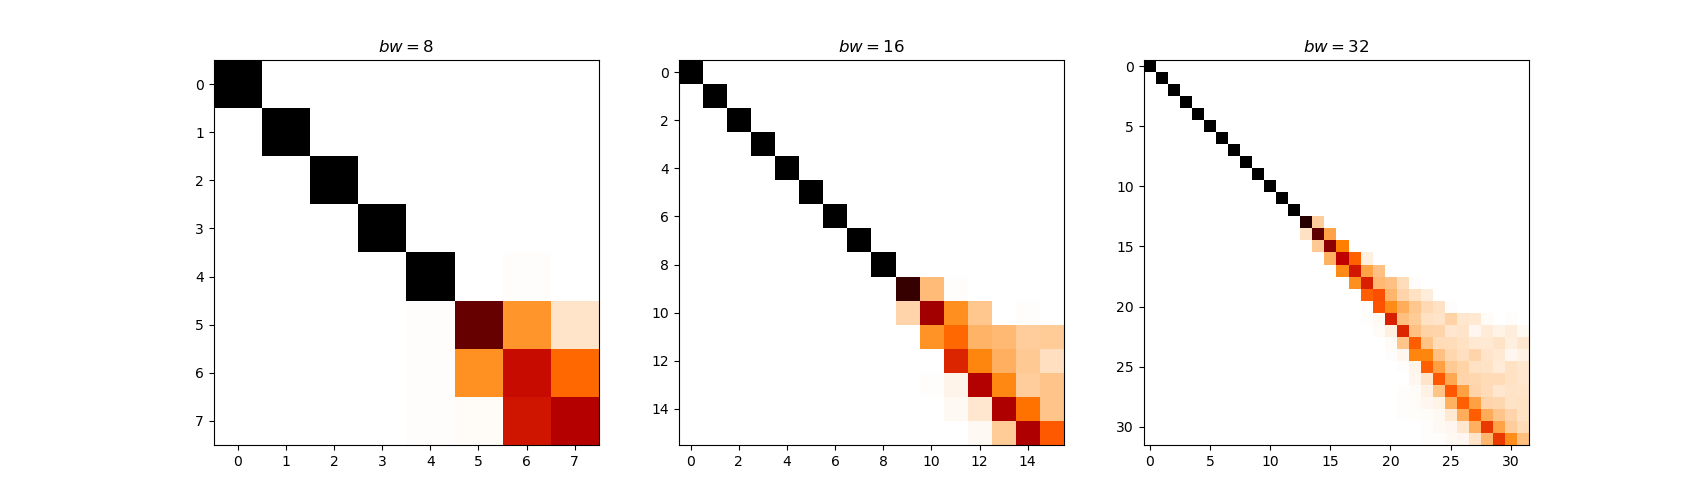
\includegraphics[width=0.9\textwidth]{../codes/03.FEM_laplacian/equiangular/mass_lumping/BL/img/linearFEM.png}
	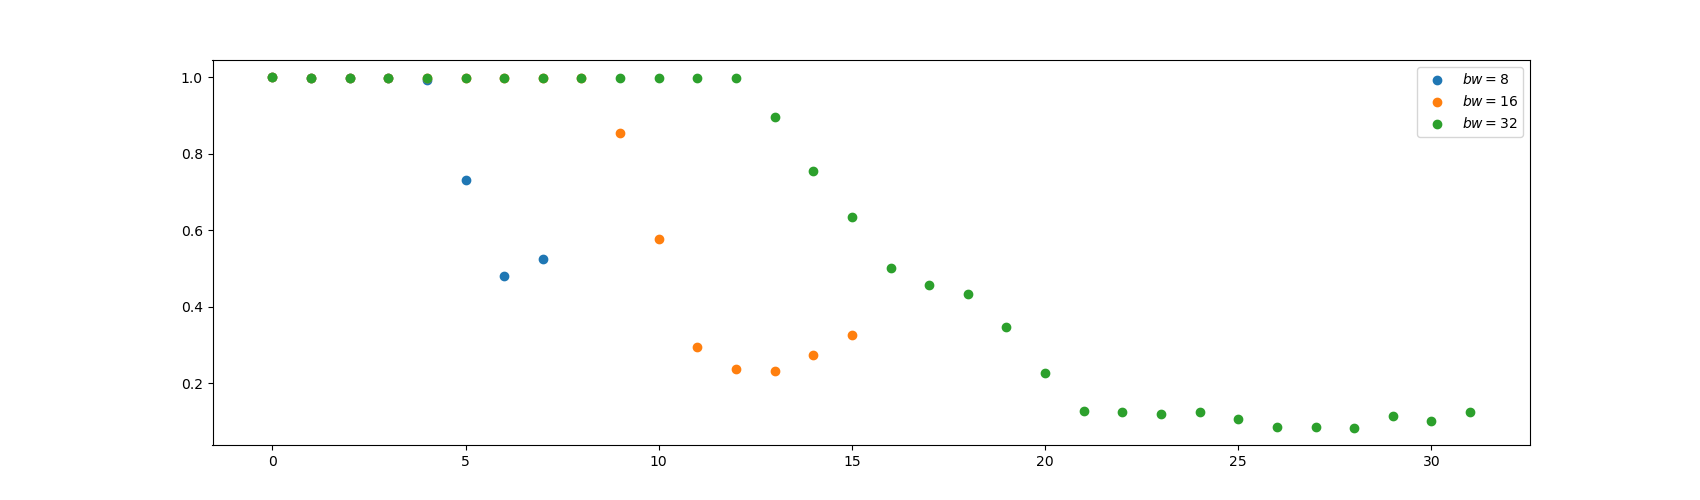
\includegraphics[width=0.9\textwidth]{../codes/03.FEM_laplacian/equiangular/mass_lumping/BL/img/linearFEM_diagonal.png}	
	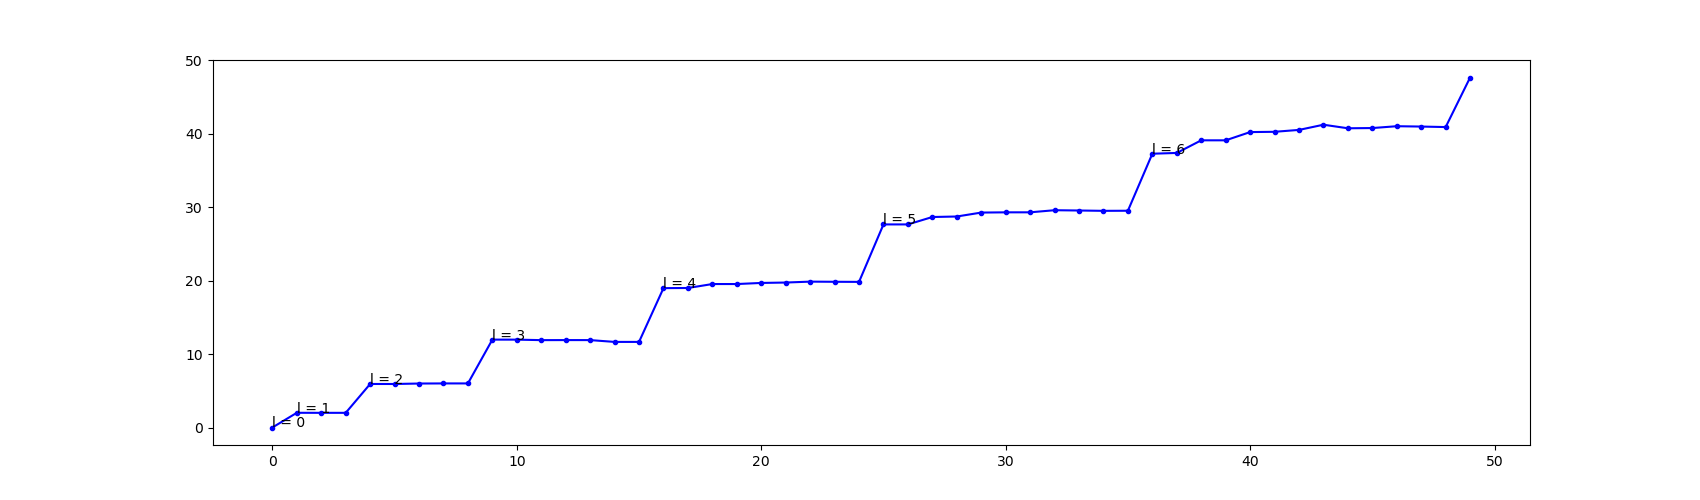
\includegraphics[width=0.9\textwidth]{../codes/03.FEM_laplacian/equiangular/mass_lumping/BL/img/FEM_eigenvalues_32.png}	
\end{figure}

\begin{figure}[h]
	\label{fig:symmetricFEMequiangularLumped}
	\caption{Symmetric Lumped Linear FEM Laplacian on equiangular sampling}
	\centering
	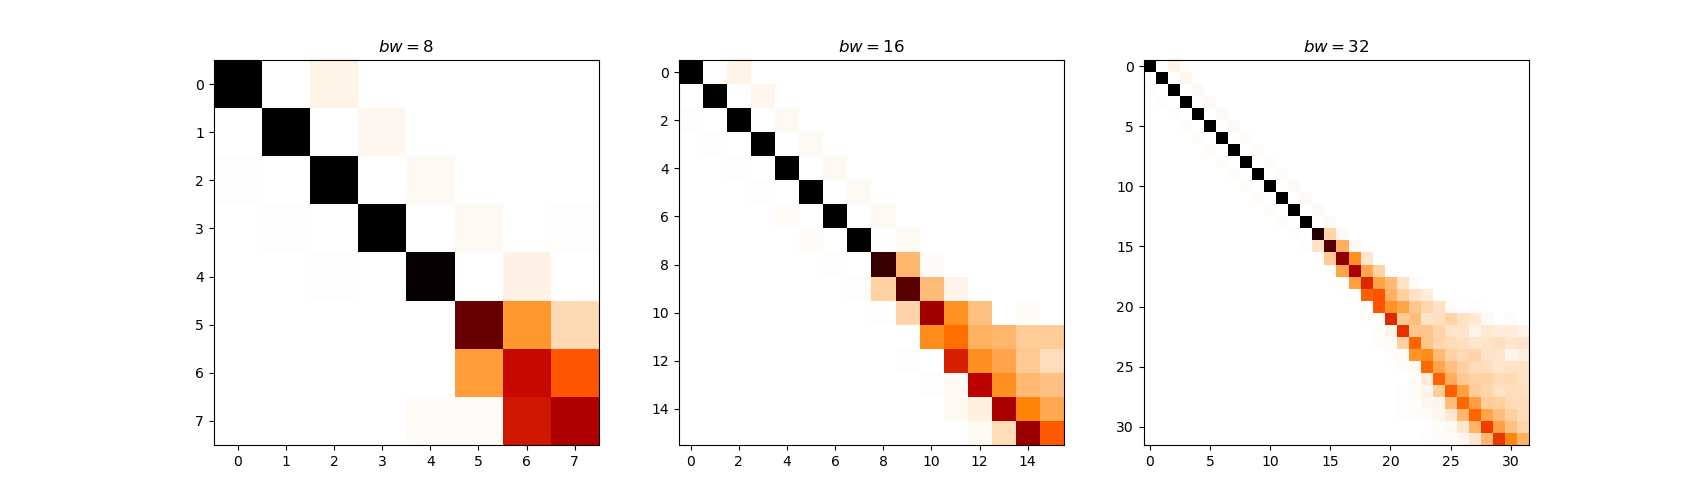
\includegraphics[width=0.9\textwidth]{../codes/03.FEM_laplacian/equiangular/mass_lumping/BLB/img/linearFEM.png}
	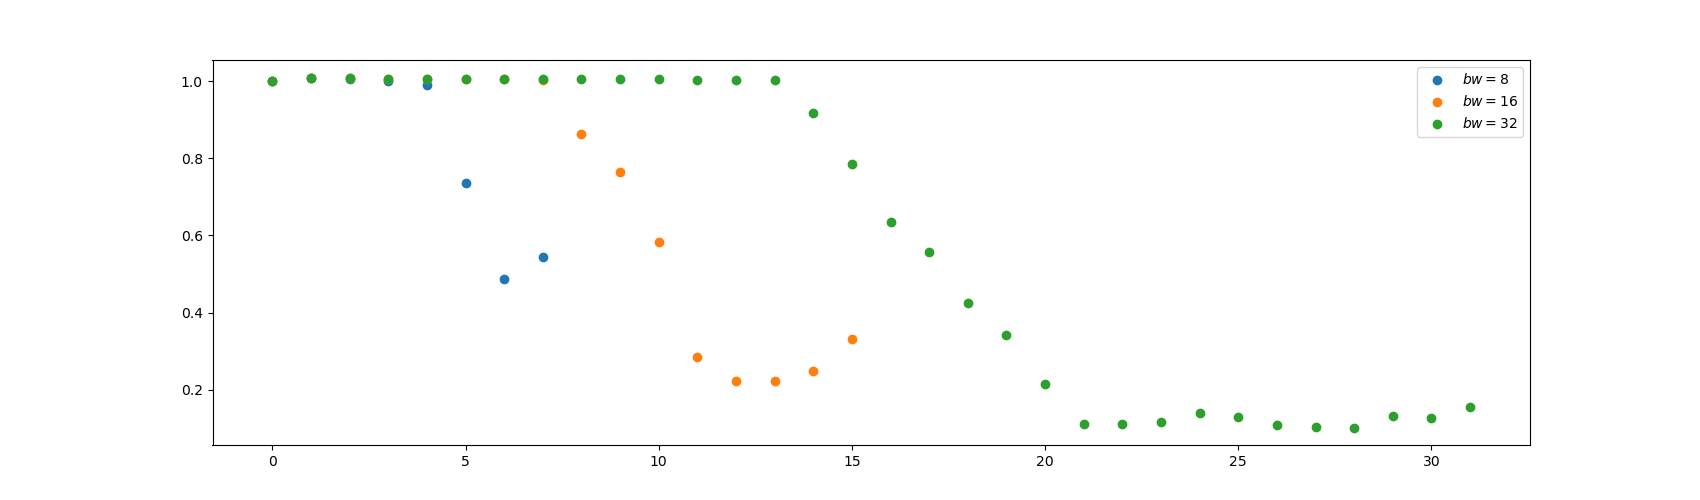
\includegraphics[width=0.9\textwidth]{../codes/03.FEM_laplacian/equiangular/mass_lumping/BLB/img/linearFEM_diagonal.png}	
	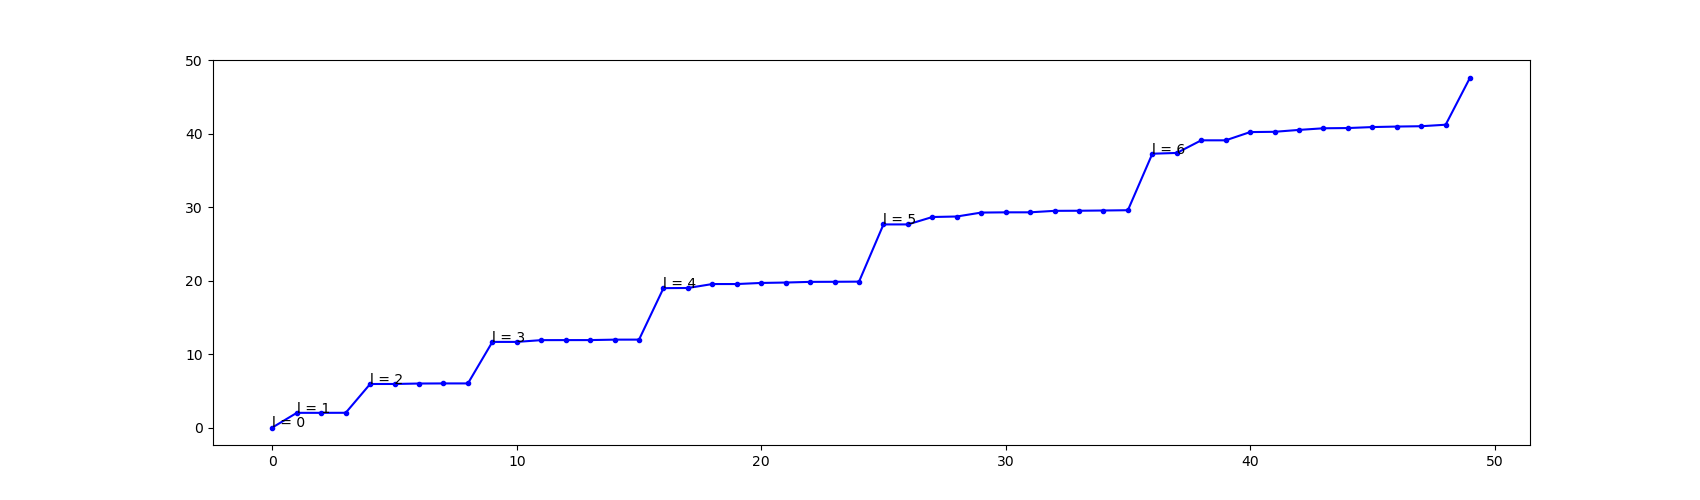
\includegraphics[width=0.9\textwidth]{../codes/03.FEM_laplacian/equiangular/mass_lumping/BLB/img/FEM_eigenvalues_32.png}	
\end{figure}
\subsubsection{Diffusion with the exponential matrix}

\paragraph{HEALPix}
\begin{figure}[h]
	\label{fig:FEM and graph diffusion on HEALPix}
	\caption{linear FEM and HKGL diffusion on HEALPix}
	\centering
	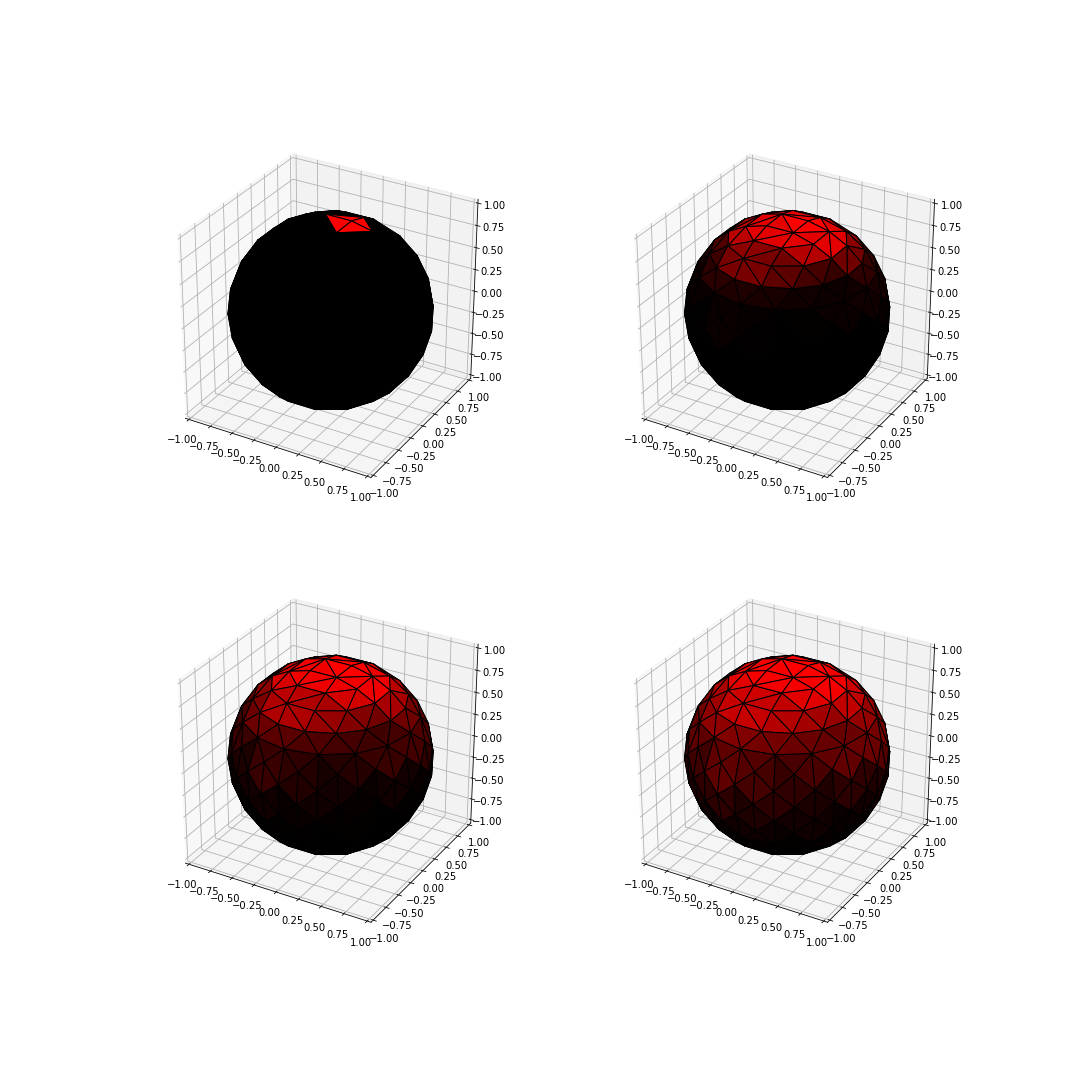
\includegraphics[width=0.6\textwidth]{../codes/03.FEM_laplacian/HEALPix/17_diffusion_img/FEM_diffusion.png}
	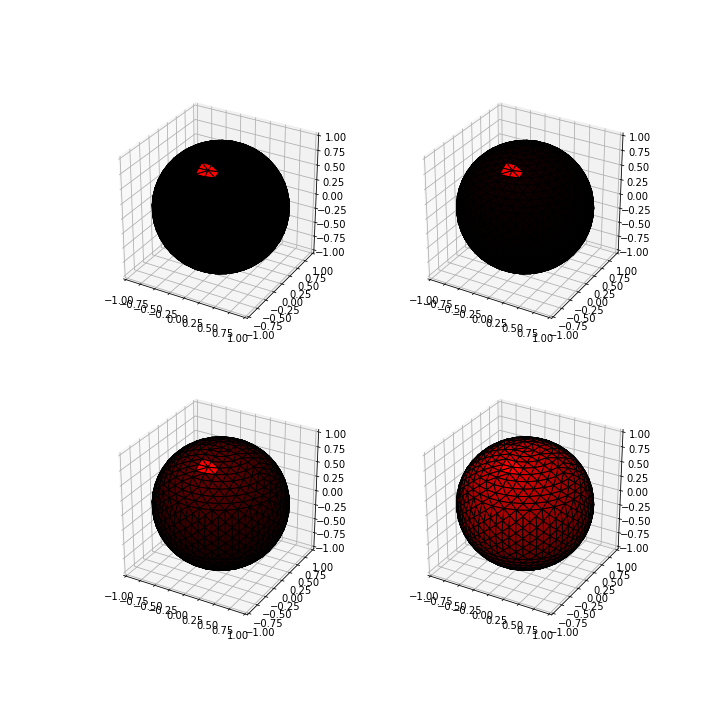
\includegraphics[width=0.6\textwidth]{../codes/03.FEM_laplacian/HEALPix/17_diffusion_img/GRAPH_diffusion.png}	
\end{figure}
\paragraph{Equiangular}
\begin{figure}[h]
	\label{fig:FEM and graph diffusion on equiangular sampling}
	\centering
	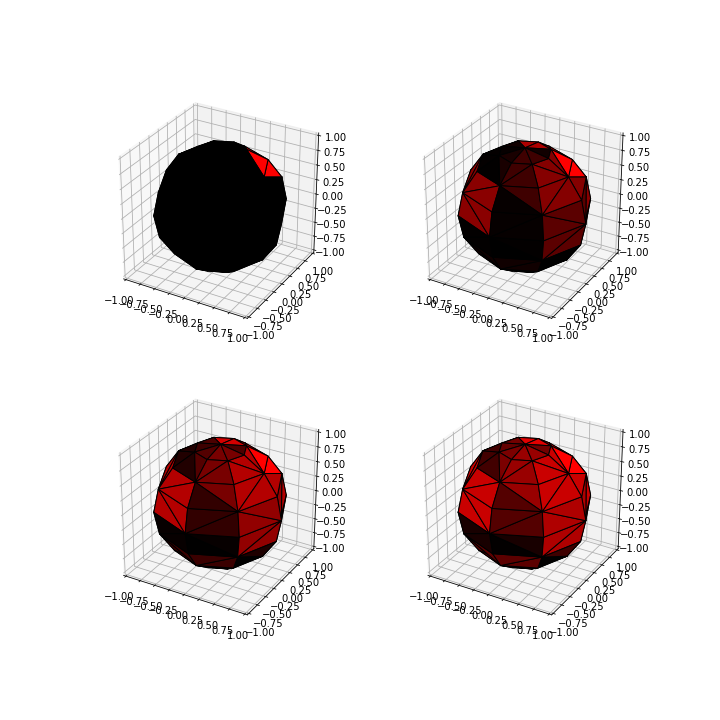
\includegraphics[width=0.6\textwidth]{../codes/03.FEM_laplacian/equiangular/normal/17_diffusion_img/FEM_diffusion.png}
	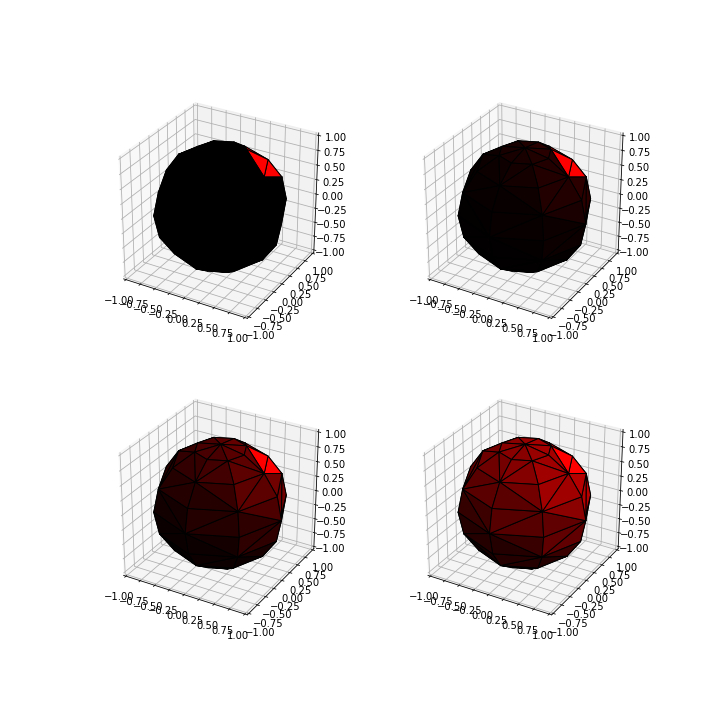
\includegraphics[width=0.6\textwidth]{../codes/03.FEM_laplacian/equiangular/normal/17_diffusion_img/GRAPH_diffusion.png}
	\caption{FEM and HKGL diffusion on equiangular sampling}
\end{figure}
\paragraph{Lumped mass matrix}

\begin{figure}[h]
	\label{fig:FEM diffusion on equiangular sampling}
	\centering
	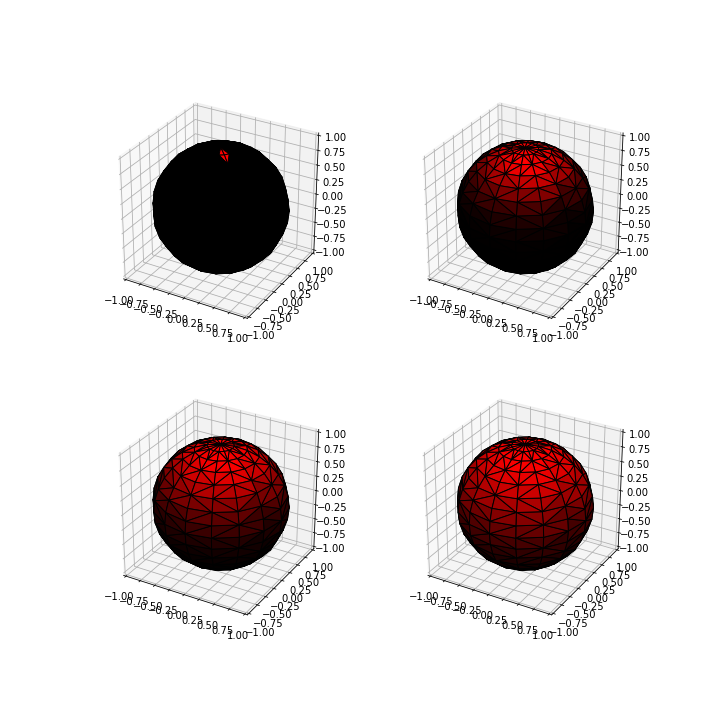
\includegraphics[width=0.4\textwidth]{../codes/03.FEM_laplacian/equiangular/mass_lumping/BL/img/FEM_diffusion.png}
	\caption{ FEM diffusion on equiangular sampling}
\end{figure}
\begin{figure}[h]
	\label{fig:FEM lumped diffusion on equiangular sampling}	
	\centering
	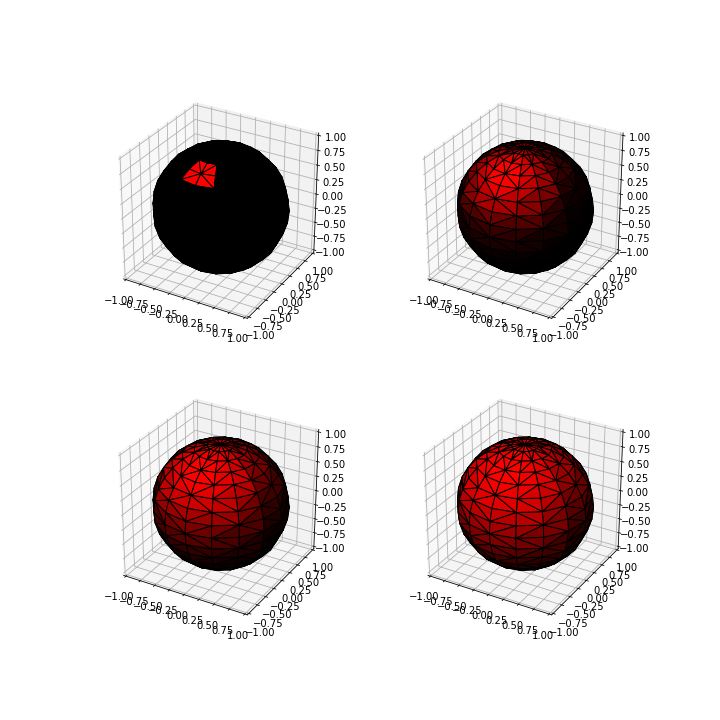
\includegraphics[width=0.4\textwidth]{../codes/03.FEM_laplacian/equiangular/mass_lumping/BL/img/FEM_lumped_diffusion.png}	
	\caption{Lumped FEM diffusion on equiangular sampling}
\end{figure}
\begin{figure}[h]
	\label{fig:FEM lumped symmetric diffusion on equiangular sampling}
	\centering
	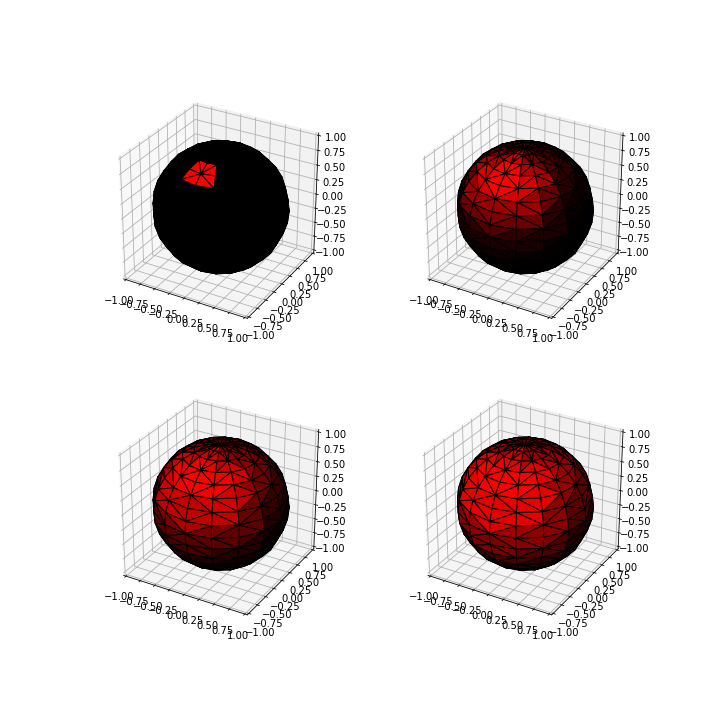
\includegraphics[width=0.4\textwidth]{../codes/03.FEM_laplacian/equiangular/mass_lumping/BL/img/FEM_lumped_symmetric_diffusion.png}
	\caption{Lumped symmetric FEM diffusion on equiangular sampling}
\end{figure}

\subsubsection{Equivariance error}

\begin{figure}[h]
	\label{fig:FEM equivariance error}
	\centering
	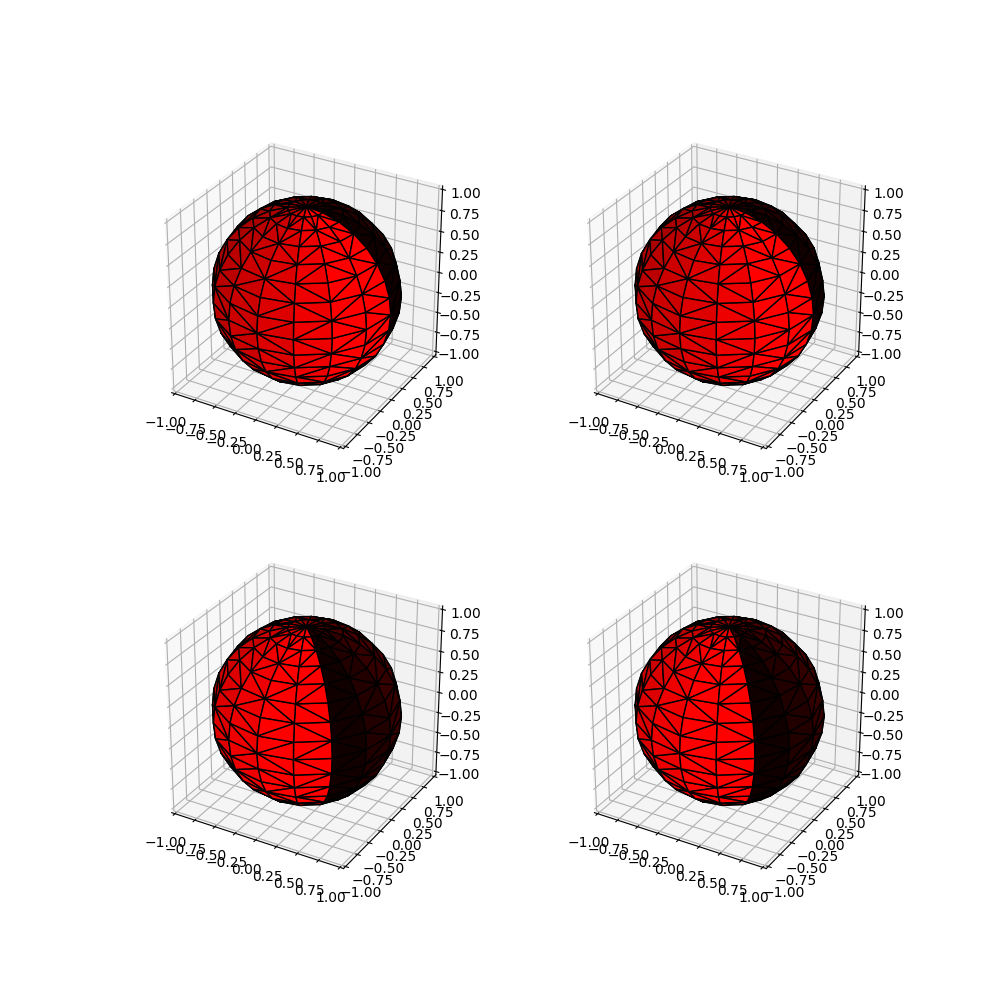
\includegraphics[width=0.6\textwidth]{../codes/03.FEM_laplacian/equiangular/normal/img/equivariance_error_FEM.png}
	\caption{FEM equivariance error}
\end{figure}
\begin{figure}[h]
	\label{fig:GRAPH equivariance error}
	\centering
	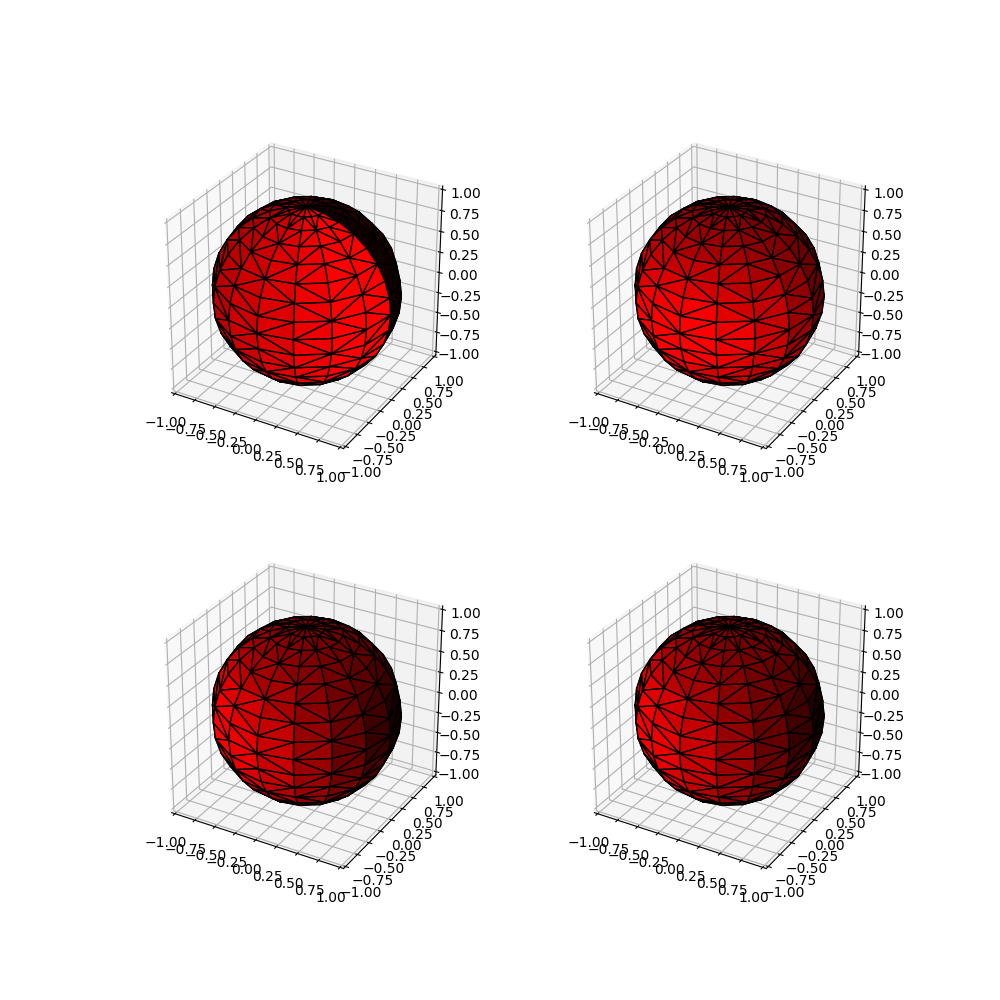
\includegraphics[width=0.6\textwidth]{../codes/03.FEM_laplacian/equiangular/normal/img/equivariance_error_GRAPH.png}
	\caption{Graph equivariance error}
\end{figure}





\pagebreak


%*******************************************************************************
%*********************************** Conclusions ***************************
%*******************************************************************************
%!TEX root = 0.main.tex

\section{Conclusions}\label{sec:Chapter4}




\subsection{Experimental validation: SHREC17}
\label{sec:Chapter5:Experimental validation}
Gusset et al. \cite{Gusset} implemented the graph proposed in this work in a GCNN and three other rotation equivariant neural networks on a popular classification problem \cite{SHREC17}. The four models tested were the following: the original version of DeepSphere, Deepsphere \textit{Optimal} - obtained implementing the thresholding procedure described in this work in section \ref{sec:Chapter2:How to build a good graph} - and the traditional SCNNs of Cohen et al. \cite{SCNN} introduced in section \ref{sec:Chapter1:SCNN} and of Esteves et al. \cite{Esteves}
\paragraph{On the Equiangular sampling}. They compare with two different metrics  (accuracy, F1-score) the performances of these four rotation invariant models, while also comparing the speed of inference and of training of each model. Results are shown in table \ref{tab:SHREC17_class}.  It can be seen how \textit{DeepSphere Optimal} has \textit{always} the highest score between all the rotation equivariant models, no matter the evaluation metric. Furthermore, its performances in terms of speed of inference and training are second only to DeepSphere, remaining by far faster than the other two SCNNs. 
\begin{table}[ht]
	\centering
	\begin{tabular}{l|c c r r r}
		\multicolumn{1}{l}{} & \multicolumn{2}{c}{performance} & \multicolumn{1}{c}{size} & \multicolumn{2}{c}{speed}\\
		\cmidrule(lr){2-3} \cmidrule(lr){4-4} \cmidrule(lr){5-6}
		\multicolumn{1}{l}{Method} & Accuracy & F1-score & params & inference & training \\ \hline
		Cohen \emph{s2cnn\_simple} & 78.59 & 78.85 & 400k & 12ms & 32h\\
		Esteves \emph{sphericalcnn} & 79.18 & 79.36 & 500k & 9.8ms & 2h52\\ \hline
		Deepsphere & 73.36 & 73.67 & 190k & \textbf{0.98ms} & \textbf{43m} \\
		\textbf{Deepsphere \emph{Optimal}} & \textbf{80.42} & \textbf{80.65} & 190k & 1.0ms & 48m
	\end{tabular}
	\caption{Results form \cite{Gusset}. Performances of four rotation equivariant GCNNs and two SCNNs on the popular classification task SHREC17.}
	\label{tab:SHREC17_class}
\end{table}
\paragraph{On HEALPix }
Gusset et al. repeated the same test on the same dataset on a HEALPix sampling with $N_{side}=32$. Results can be seen in table \ref{table:results}.
\begin{table}[h!]
	\centering
	\begin{tabular}{ c|c|c } 
		& DeepSphere & DeepSphere \textit{Optimal} \\ 
		\hline
		accuracy & 82.23\% & 82.76\% \\ 
	\end{tabular}
	\caption{\label{table:results}Results form Gusset et al. Accuracy on the HEALPix sampling}
\end{table}
Being the new graph of DeepSphere Optimal more equivariant to rotations, we expected to see an improvement in the accuracy, as we did in the equiangular case. The fact that this improvement was not observed on HEALPix means that, in this case, the original DeepSphere graph $W$ \textit{is already sufficiently equivariant to rotations}. By this we mean that for this task, being equivariant to rotations of the low frequency eigenmodes is sufficient to obtain good results, and that being rotation equivariant to the higher frequencies does not lead to any improvement.

\subsection{Confront of different Discrete Laplacians on the equiangular sampling}
We conclude by showing how the different discrete Laplacians $\mathbf L$ illustrated so far compare in terms of equivariance error and computational time of the filter $\mathcal F(\mathbf f) = \mathbf L\mathbf f$. We can see how the three sparse discrete Laplacians are one order of magnitude faster than the two full Laplacians. The FEM approach is actually able to reduce the equivariance error compared to the HKGL, and it stays low even when using the sparse, lumped approximation $B^{-1}A$. The lumped FEM Laplacian $D^{-1}A$ performs really well, and gets close to the performances of the graph Laplacian of Khasanova and Frossard. 
\begin{figure}[h!]
	\centering
	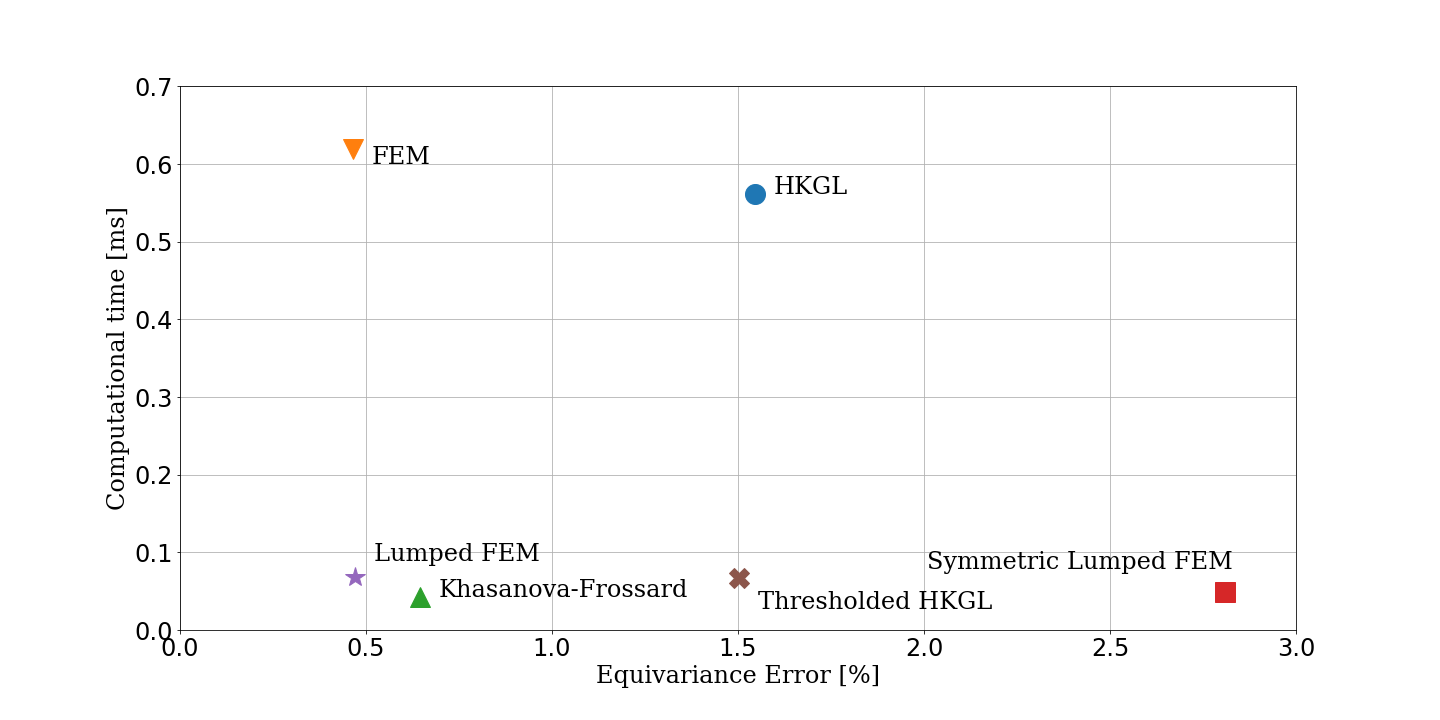
\includegraphics[width=\textwidth]{../codes/06.Equivariance_error/tradeoff.png}
	\caption{\label{fig:tradeoff}Trade-off between computational time and equivariance error for the filter $\mathbf L$ for different discrete Laplacians on the equiangular sampling}
\end{figure}

\subsection{Final considerations and future work}


Having a metric means using a \textit{non-symmetric matrix} $B^{-1}A$ such that the generalized eigenvalue problem $Av = \lambda B v$ is such that $v_i$ approximates the corresponding sampled SH and $VBV^T=I$. With a graph this is not possible since we restrict ourself to \textit{symmetric} Laplacians and thus make it impossible to incorporate a metric $B$, since the symmetry of $L$ imposes $VV^T=I$. However, there are good approximations that even by being symmetric perform well: the Khasanova-Frossard graph is an example. Further research would be 

\pagebreak

\bibliography{references.bib} 

\nocite{*}

\pagebreak



\end{document}
